 
%\subsection{Ratio Method: Run 2 EOY \& UL Resolutions}

Time resolutions were produced with the Ratio method for both EOY and UL MiniAOD datasets in 2018, 2017, and 2016 of Run 2 as shown in Figure~\ref{678EOYres}. Results for Run 2 EOY where produced for 2018 with CMSSW 10.2.5 using GT 102X\_dataRun2\_v15 from the EGamma stream given below. For 2016 and 2017 the results where produced with CMSSW 9.4.10 using GT 94X\_dataRun2\_v10 from the DoubleEG streams as detailed below.

\begin{center}
\begin{tabular}{ c c c }
 2018 EGamma & 2017 DoubleEG & 2016 DoubleEG \\
 Run2018A-17Sep2018-v2 & Run2017B-31Mar2018-v1 & Run2016B-17Jul2018\_ver2-v1\\
 Run2018B-17Sep2018-v1 & Run2017C-31Mar2018-v1 & Run2016C-17Jul2018-v1 \\
 Run2018C-17Sep2018-v1 & Run2017D-31Mar2018-v1 & Run2016D-17Jul2018-v1 \\
 Run2018D-22Jan2019-v2 & Run2017E-31Mar2018-v1 & Run2016E-17Jul2018-v1 \\
                       & Run2017F-31Mar2018-v1 & Run2016F-17Jul2018-v1 \\
                       &                       & Run2016H-17Jul2018-v1
\end{tabular}
\end{center}

%Resolutions for Same RO unit in 2018, 2017, and 2016 of Run 2 for EOY are shown separately in the left plot of Figure \ref{678EOYres}. As can be seen in the plot, 2016 and 2017 have a similar resolution of $\sim$94 ns and $\sim$91 ns respectfully while 2018 shows a larger resolution of $\sim$109 ns. In the middle plot of Figure \ref{678EOYres} different RO resolutions are shown for the same time periods. In this plot we can see that 2016 and 2017 also have similar resolutions of approximately $\sim$179 ns and $\sim$170 ns while 2018 shows a smaller resolution of $\sim$139 ns. The $Z\rightarrow e^{+}e^{-}$ resolutions for Run 2 are shown in the right plot of Figure \ref{678EOYres}, in which we can see that 2016 and 2017 have resolutions of $\sim$245 ns and $\sim$223 ns while 2018 has a much smaller resolution of $\sim$150 ns.

\begin{figure}[htbp]
\begin{center}
%\resizebox{0.48\textwidth}{!}{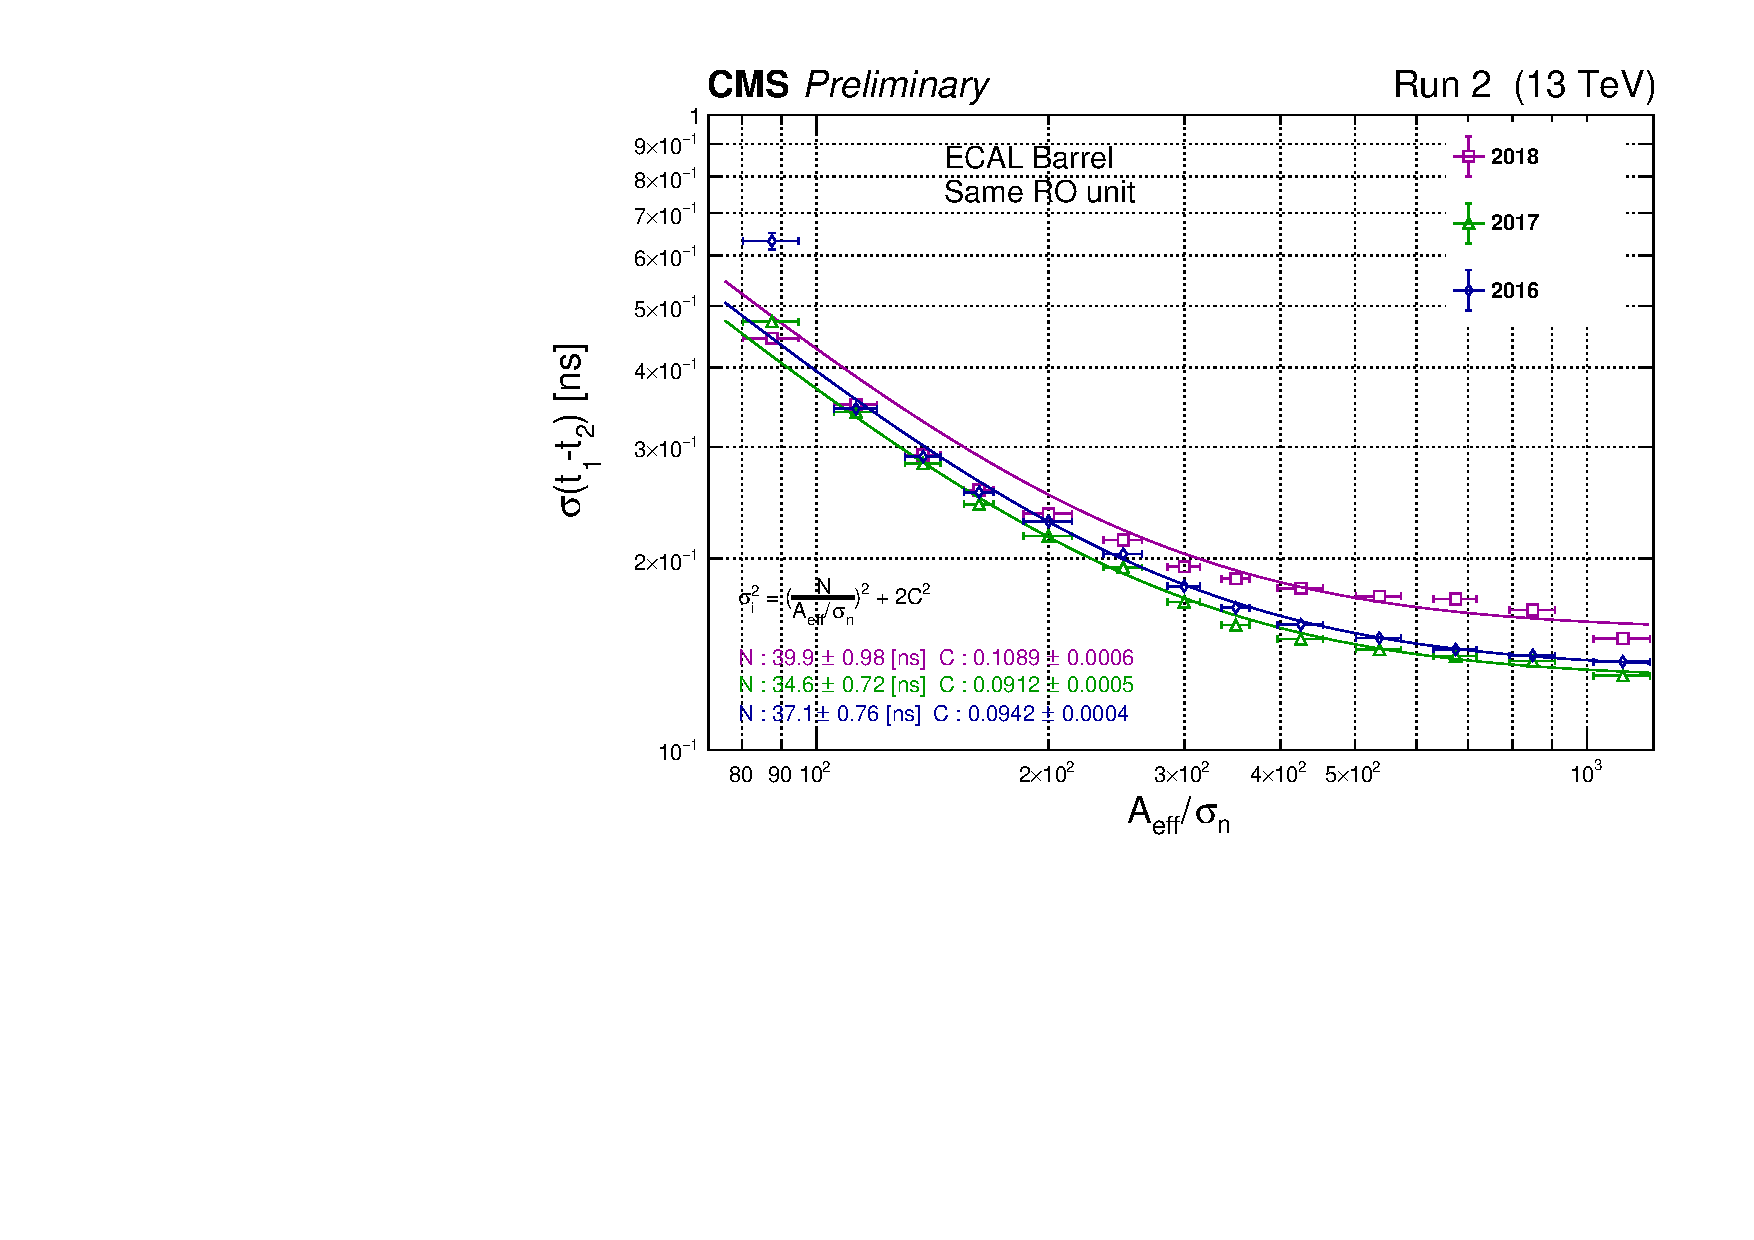
\includegraphics{fig/sec_results/tr_mini_678_loc_gt_01072020094754.pdf}}
\resizebox{0.48\textwidth}{!}{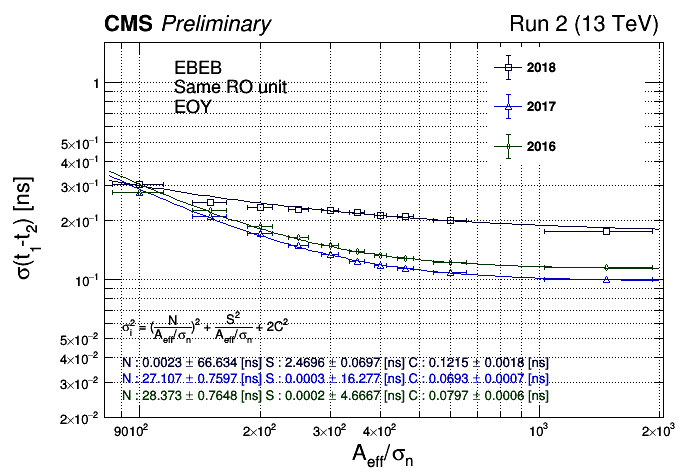
\includegraphics{fig/sec_results/tr_r2_ls_ey_13122021113951.png}}
%\resizebox{0.48\textwidth}{!}{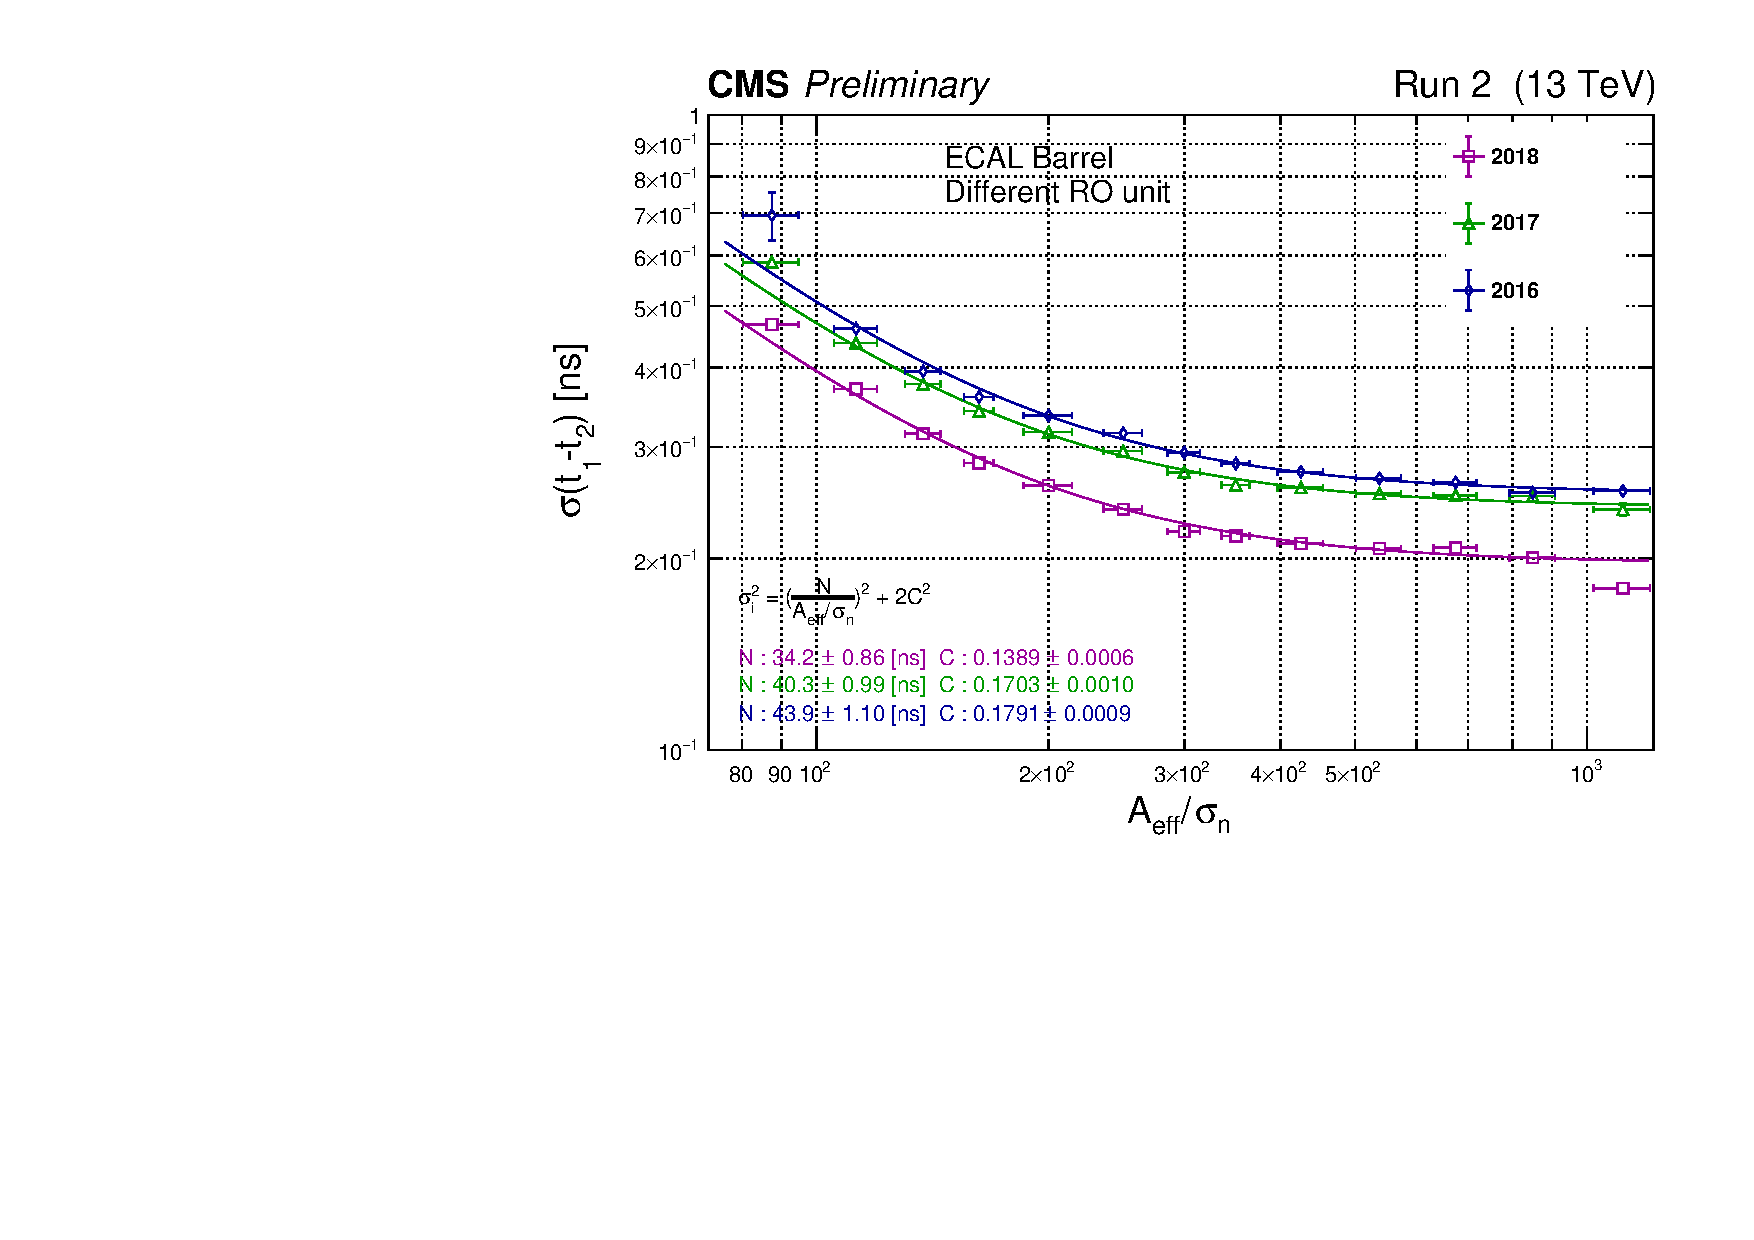
\includegraphics{fig/sec_results/tr_mini_678_locd_gt_01072020094754.pdf}}
\resizebox{0.48\textwidth}{!}{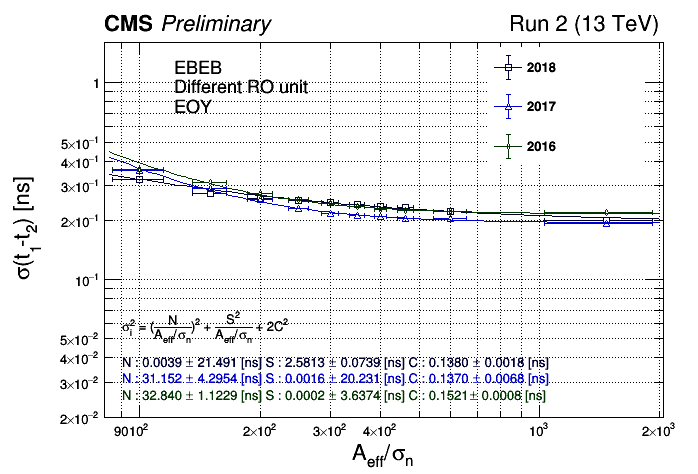
\includegraphics{fig/sec_results/tr_r2_ld_ey_13122021113951.png}}
%\resizebox{0.48\textwidth}{!}{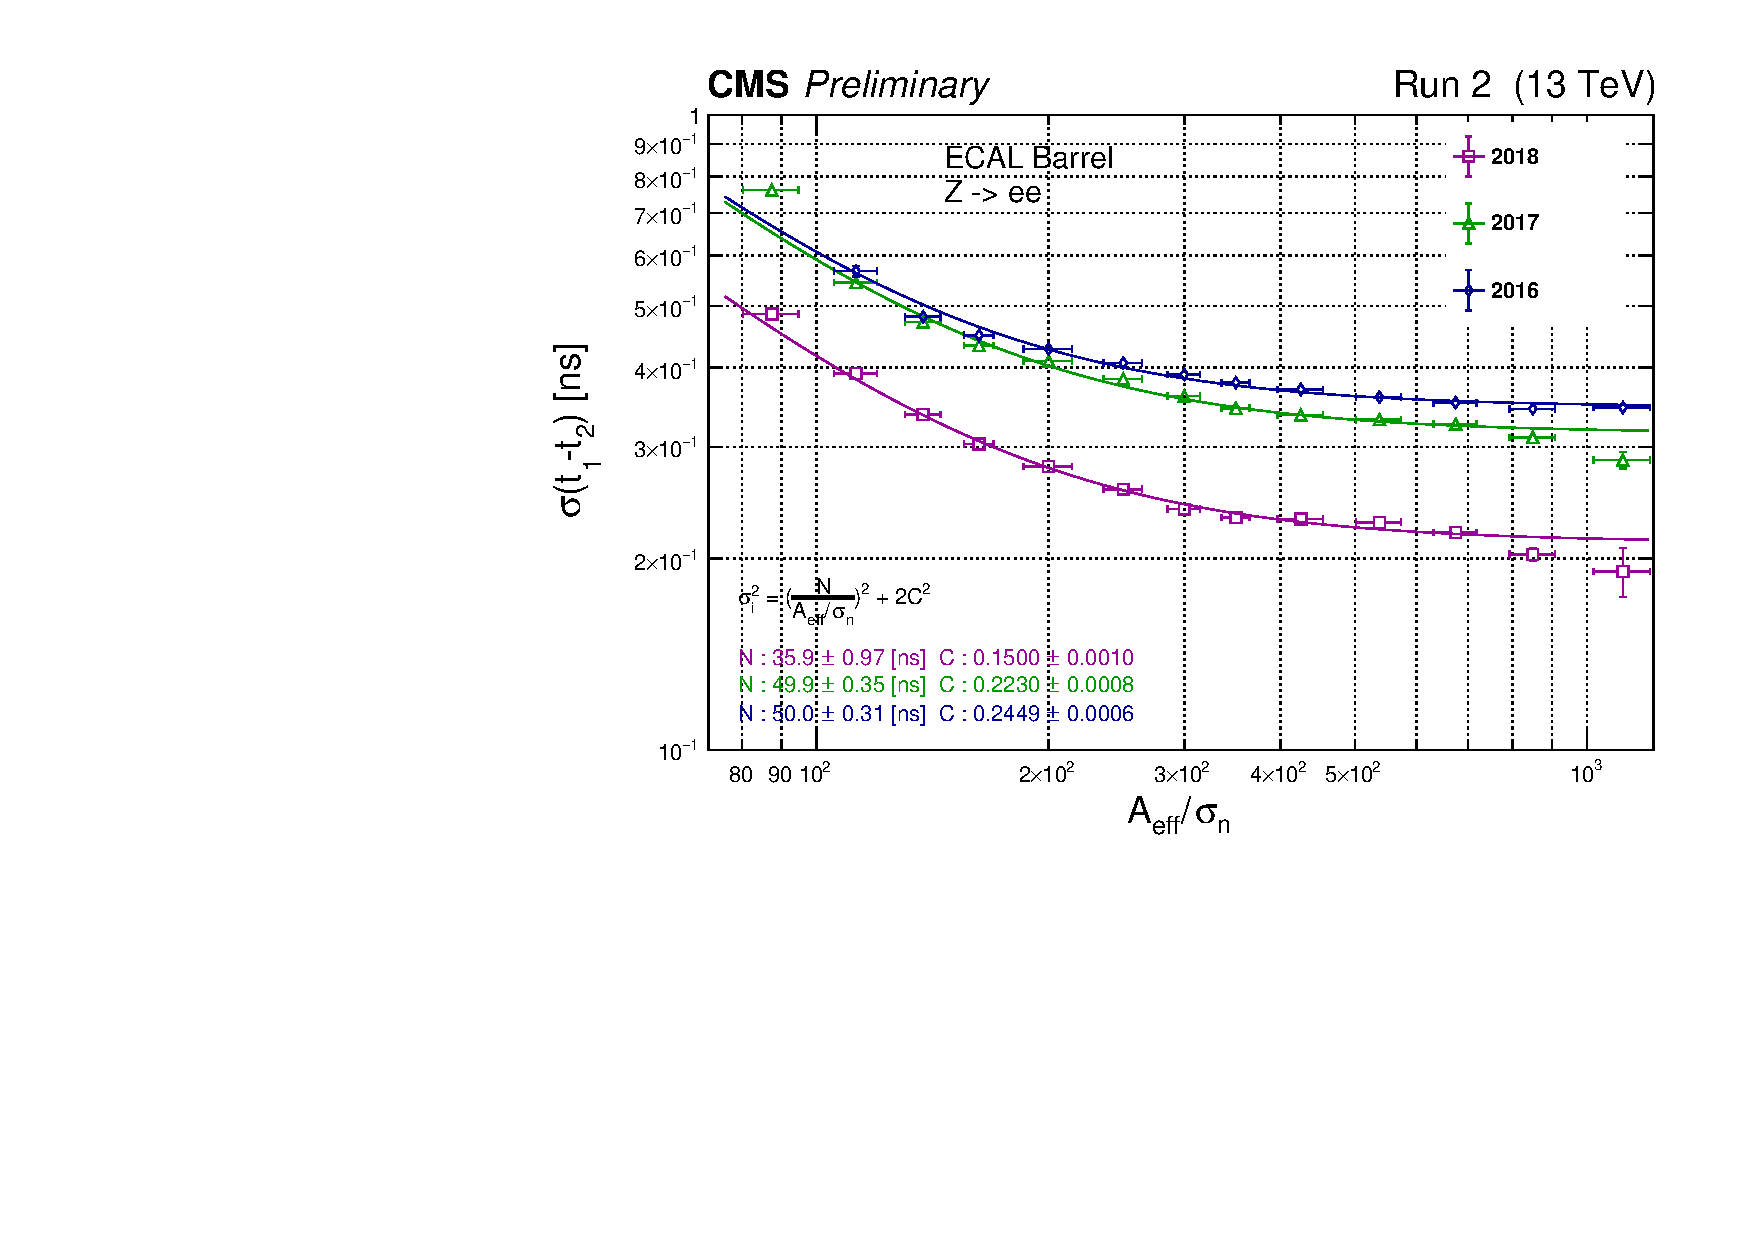
\includegraphics{fig/sec_results/tr_mini_678_glo_gt_01072020094754.pdf}}
\resizebox{0.48\textwidth}{!}{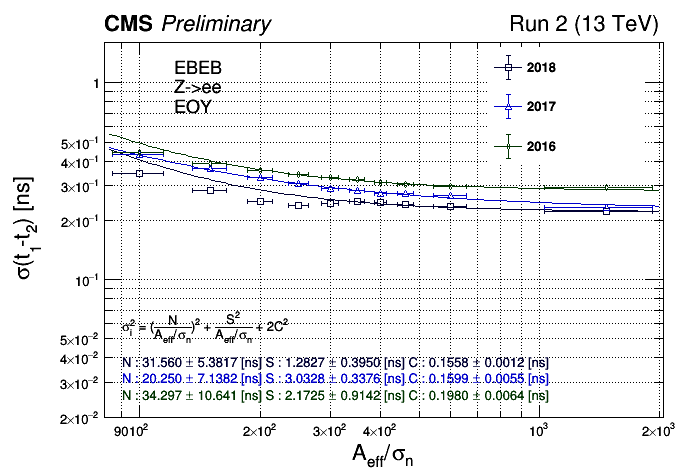
\includegraphics{fig/sec_results/tr_r2_gi_ey_13122021113951.png}}
\caption{ECAL default reconstruction same RO unit, different RO unit, and $Z\rightarrow e^{+}e^{-}$ time resolutions for End of Year Run 2 produced with the EGamma data-stream for 2018 and Double Egamma data-stream for 2017 and 2016.}
\label{678EOYres}
\end{center}
\end{figure}

%\begin{figure}[htbp]
%\begin{center}
%\resizebox{0.48\textwidth}{!}{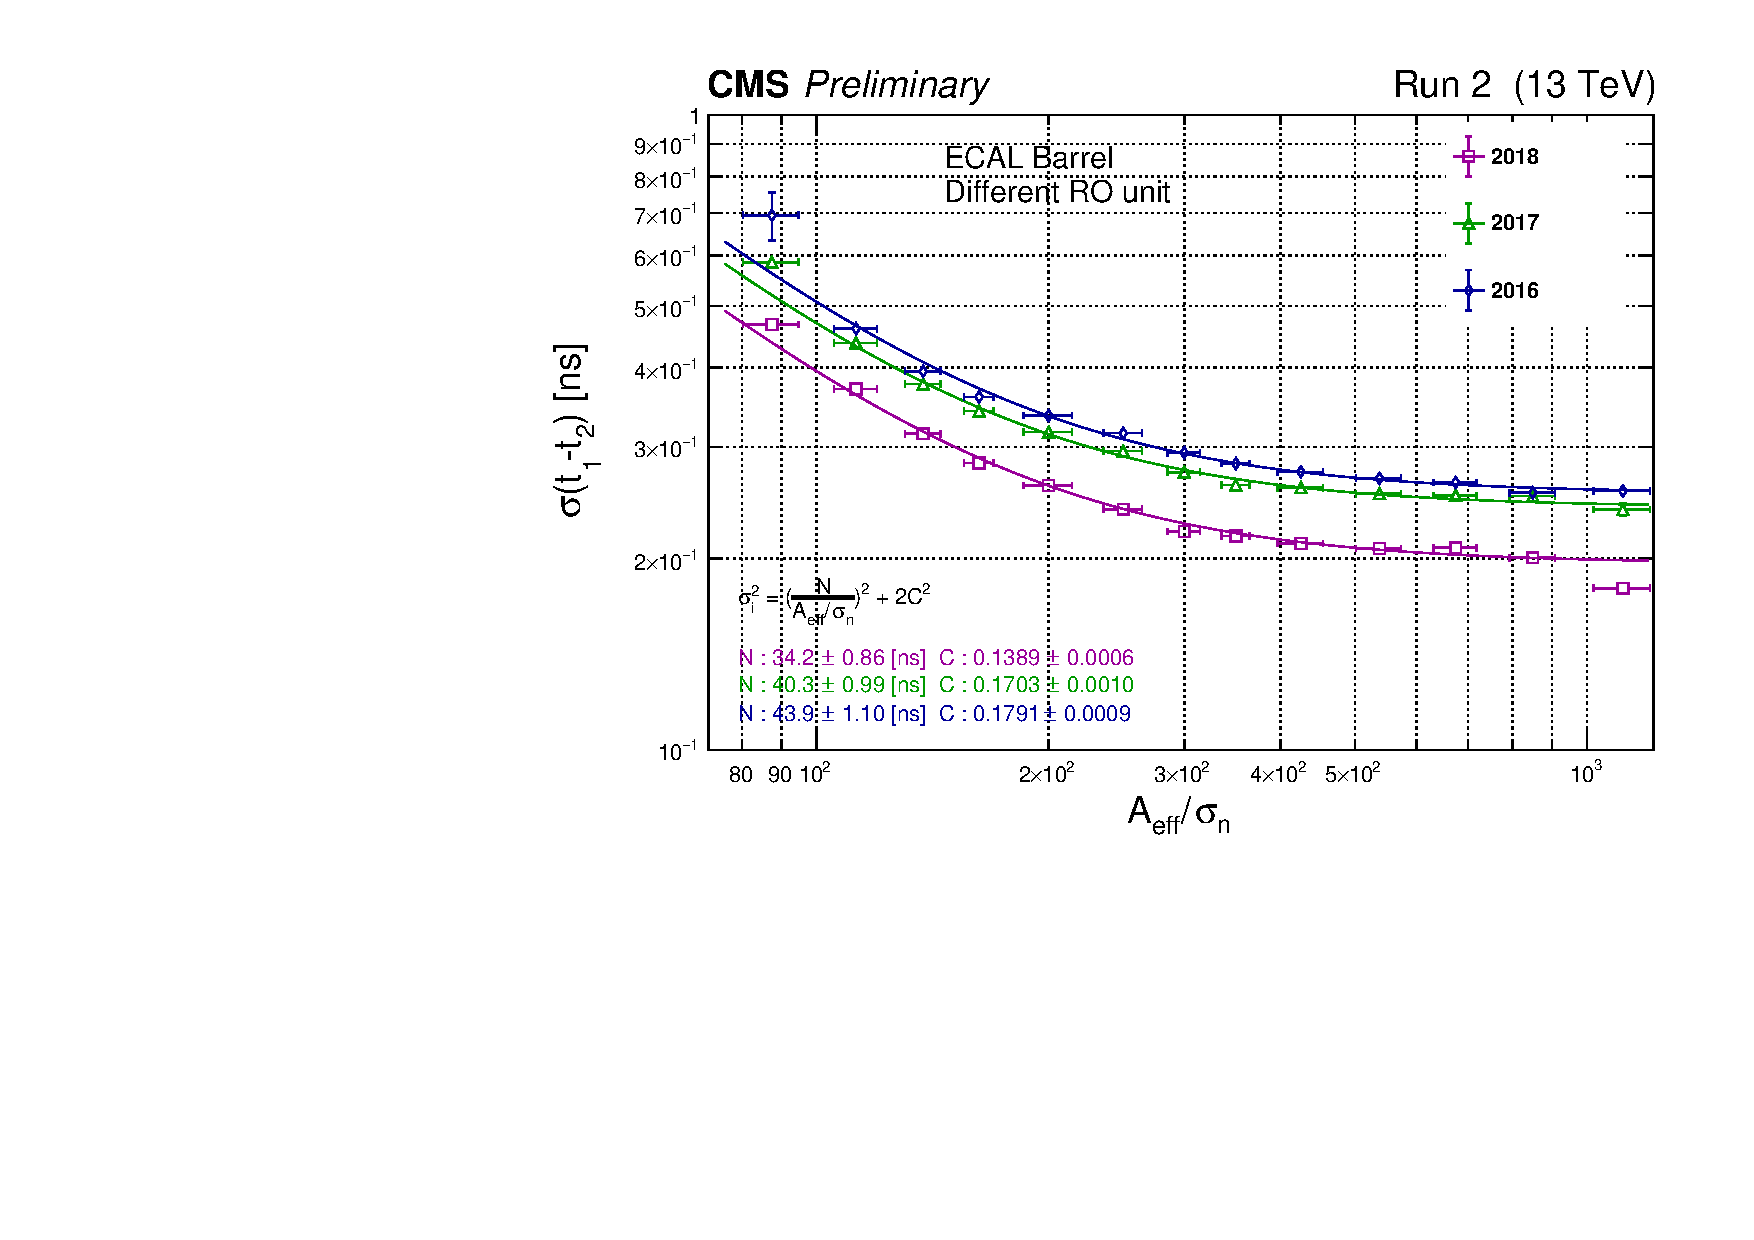
\includegraphics{fig/sec_results/tr_mini_678_locd_gt_01072020094754.pdf}}
%\caption{Different RO unit Resolution for Run 2 }
%\label{678diff}
%\end{center}
%\end{figure}

%\begin{figure}[htbp]
%\begin{center}
%\resizebox{0.48\textwidth}{!}{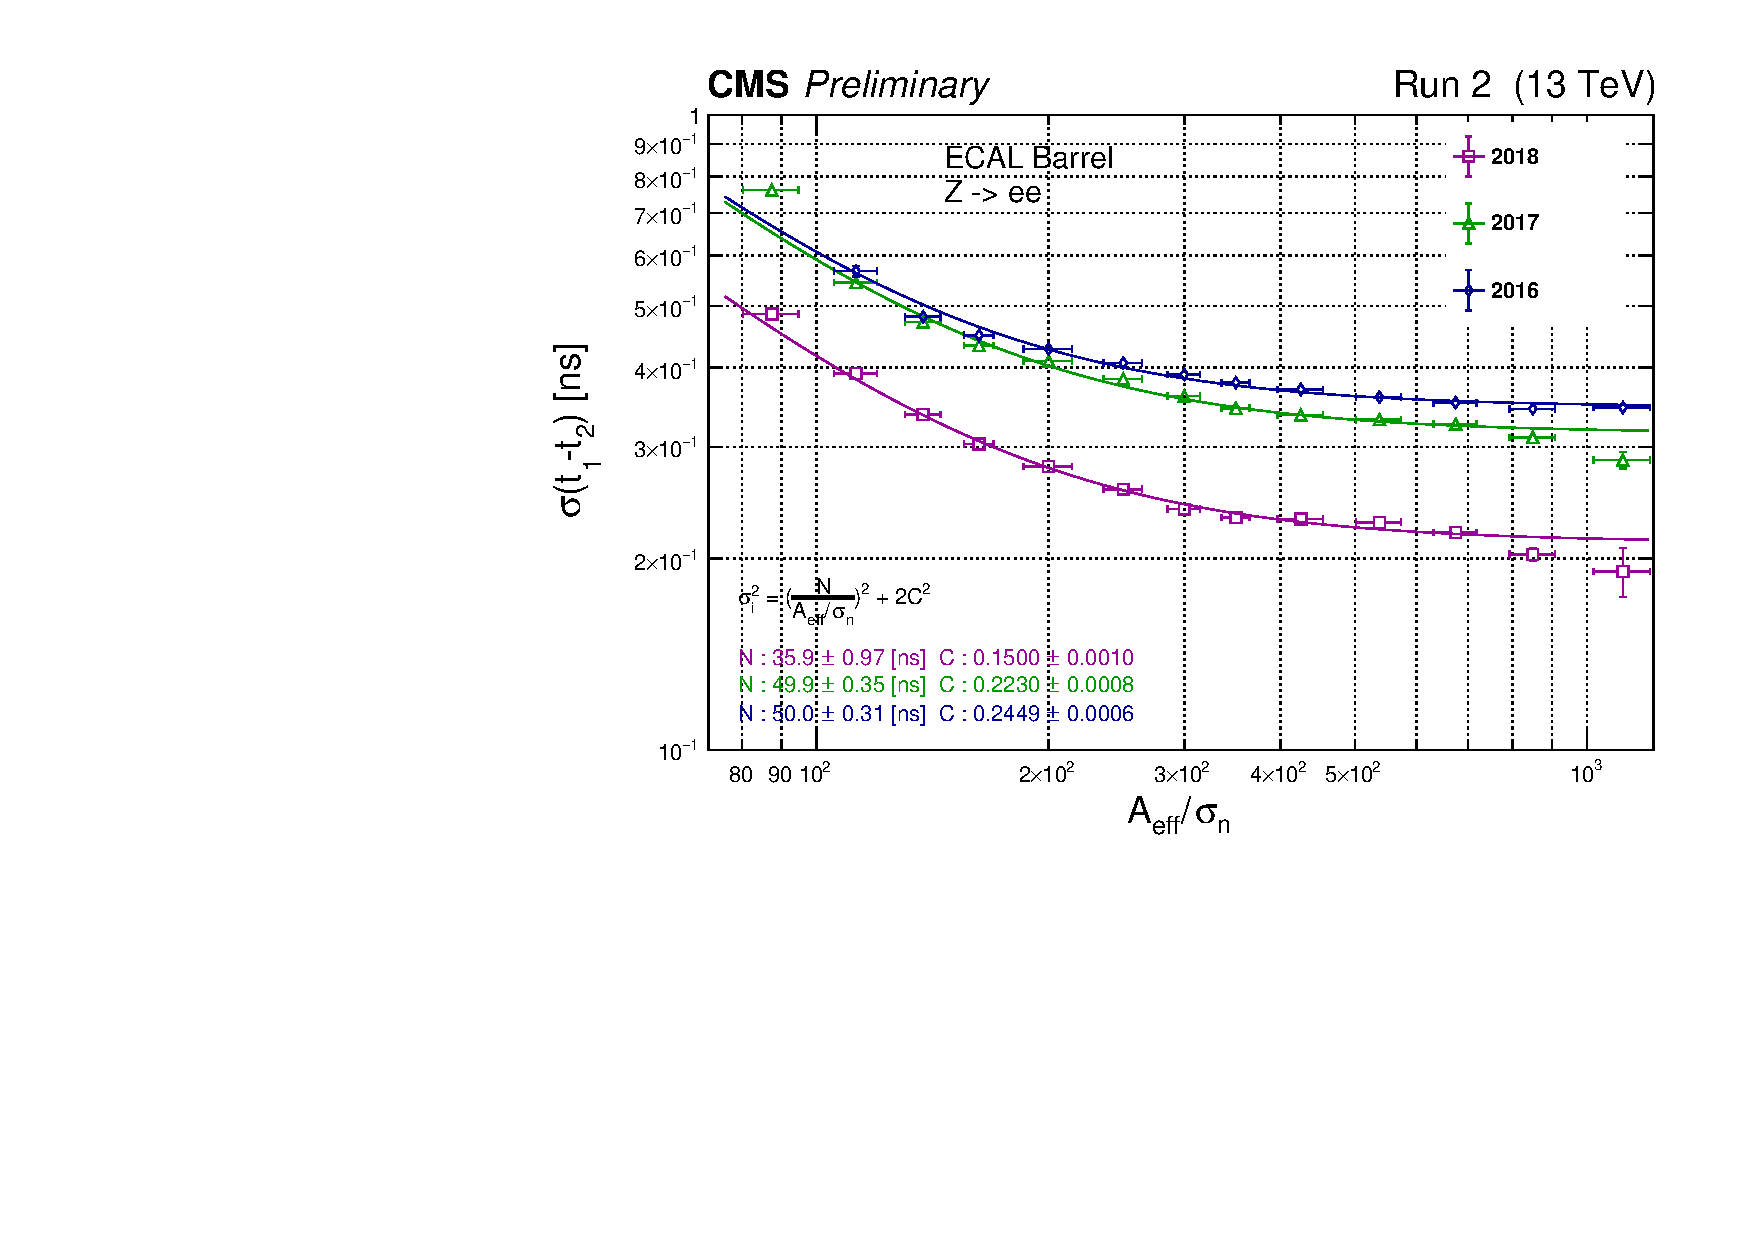
\includegraphics{fig/sec_results/tr_mini_678_glo_gt_01072020094754.pdf}}
%\caption{$Z\rightarrow e^{+}e^{-}$ Resolution for Run 2 }
%\label{678glo}
%\end{center}
%\end{figure}

%\FloatBarrier
\sloppy
The time resolution for the Run 2 UL datasets, shown in Figure~\ref{678ULres}, where produced with CMSSW 10.6.14 using GT 106X\_dataRun2\_v27 for 2016, GT 106X\_dataRun2\_v20 for 2017, and GT 106X\_dataRun2\_v26 for 2018.  The EGamma stream is used to produce the resolutions for 2018 and the DoubleEG stream is used for 2016 and 2017 as detailed below.

\begin{center}
\begin{tabular}{ c }
%\hline
2018 EGamma \\
%\hline
Run2018A-12Nov2019\_UL2018-v2 \\
Run2018B-12Nov2019\_UL2018-v2 \\
Run2018C-12Nov2019\_UL2018-v2 \\
Run2018D-12Nov2019\_UL2018-v4 \\
%\hline
\end{tabular}
\end{center}

\begin{center}
\begin{tabular}{ c c }
%\hline
2017 DoubleEG & 2016 DoubleEG \\
%\hline
Run2017B-09Aug2019\_UL2017-v1 & Run2016B-21Feb2020\_ver2\_UL2016\_HIPM-v1 \\
Run2017C-09Aug2019\_UL2017-v1 & Run2016C-21Feb2020\_UL2016\_HIPM-v1 \\
Run2017D-09Aug2019\_UL2017-v1 & Run2016D-21Feb2020\_UL2016\_HIPM-v1 \\
Run2017E-09Aug2019\_UL2017-v1 & Run2016E-21Feb2020\_UL2016\_HIPM-v1 \\
Run2017F-09Aug2019\_UL2017-v1 & Run2016F-21Feb2020\_UL2016-v1 \\
                              & Run2016G-21Feb2020\_UL2016-v1 \\
                              & Run2016H-21Feb2020\_UL2016-v1 \\
%\hline
\end{tabular}
\end{center}

%Resolutions for Same RO unit in 2018, 2017, and 2016 of Run 2 for UL are shown separately in the left plot in Figure \ref{678ULres}. As can be seen in the plot, 2016 and 2017 have a similar resolution of $\sim$xx ns and $\sim$xx ns respectfully while 2018 shows a larger resolution of $\sim$xx ns. The middle plot in Figure \ref{678ULres} different RO resolutions are shown for the same time periods. In this plot we can see that 2016 and 2017 also have similar resolutions of approximately $\sim$xx ns and $\sim$xx ns while 2018 shows a smaller resolution of $\sim$xx ns. The $Z\rightarrow e^{+}e^{-}$ resolutions for Run 2 are shown in the right plot in Figure \ref{678ULres}, in which we can see that 2016 and 2017 have resolutions of $\sim$xx ns and $\sim$xx ns while 2018 has a much smaller resolution of $\sim$xx ns.

% !!!!!!!!! Replace UL plots with new GT resolutions - quote correct GT for 2018D UL - need to remake these plots with correct 2018D GT !!!!!!!!!!!!!!!!!!!


%\begin{figure}[htbp]
%\begin{center}
%\resizebox{0.48\textwidth}{!}{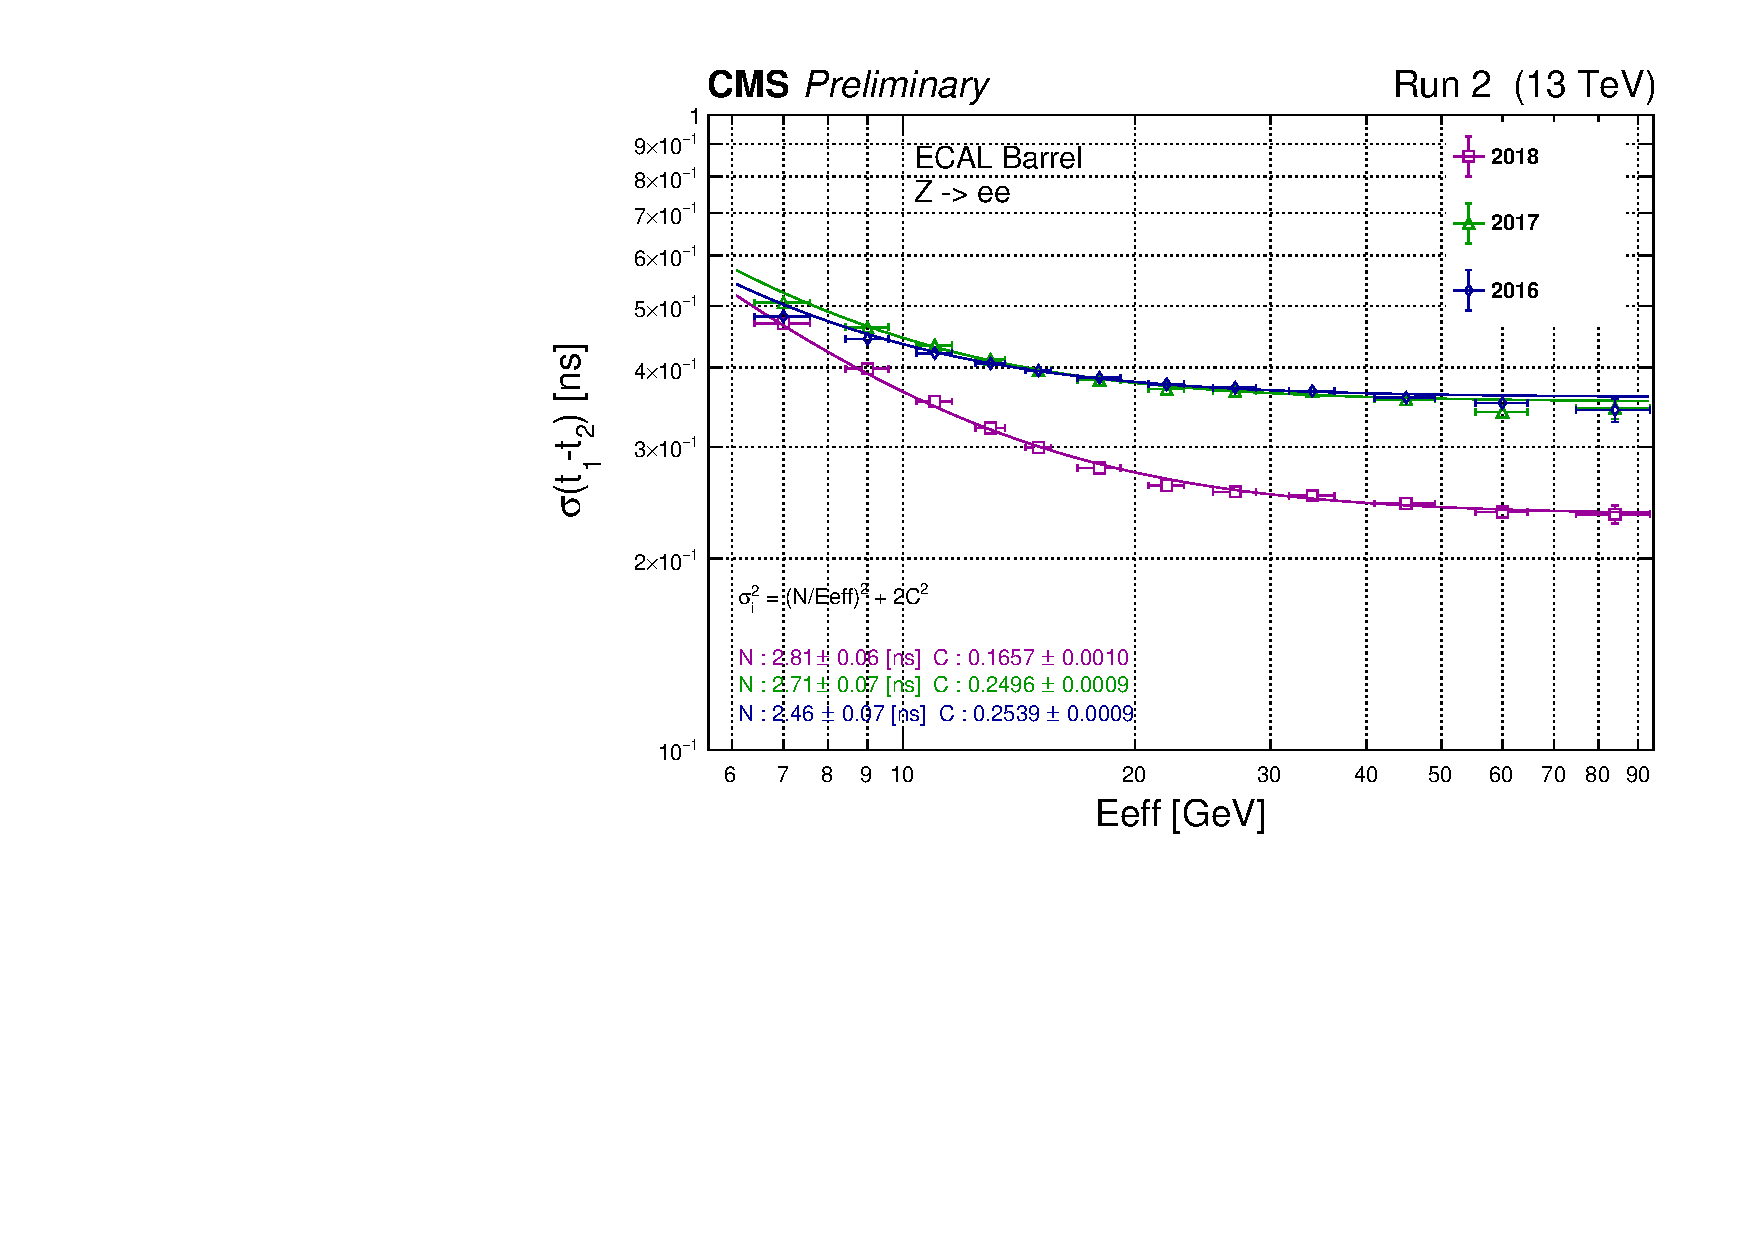
\includegraphics{fig/sec_results/tr_mini_678_Eeff_otg_01072020100707.pdf}}
%\caption{$Z\rightarrow e^{+}e^{-}$ Resolution w.r.t. effective energy for Run 2 by year}
%\label{678gloe}
%\end{center}
%\end{figure}

%\begin{figure}[htbp]
%\begin{center}
%\resizebox{0.48\textwidth}{!}{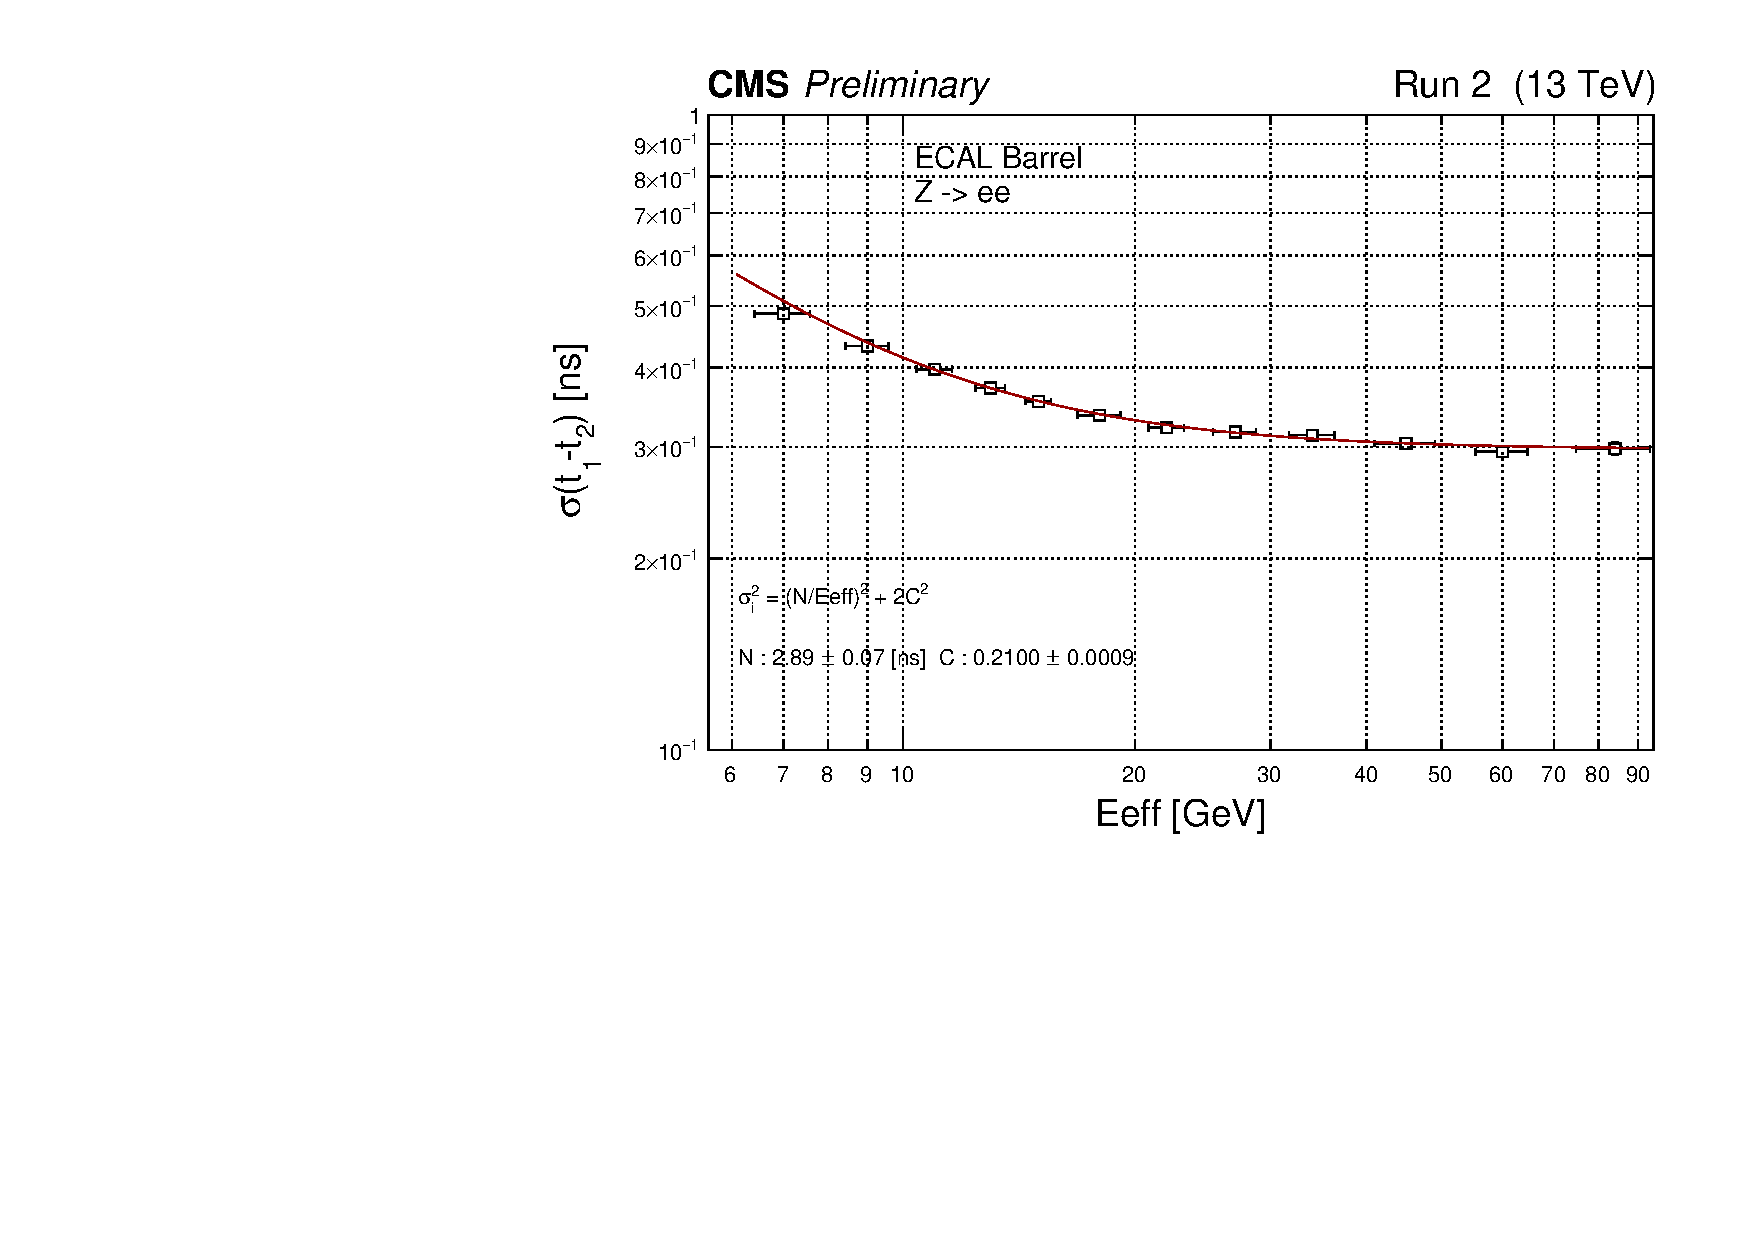
\includegraphics{fig/sec_results/tr_mini_2_Eeff_gt_01072020100906.pdf}}
%\caption{$Z\rightarrow e^{+}e^{-}$ Resolution w.r.t. effective energy for Run 2 }
%\label{2gloe}
%\end{center}
%\end{figure}

%\begin{figure}[htbp]
%\begin{center}
%\resizebox{0.48\textwidth}{!}{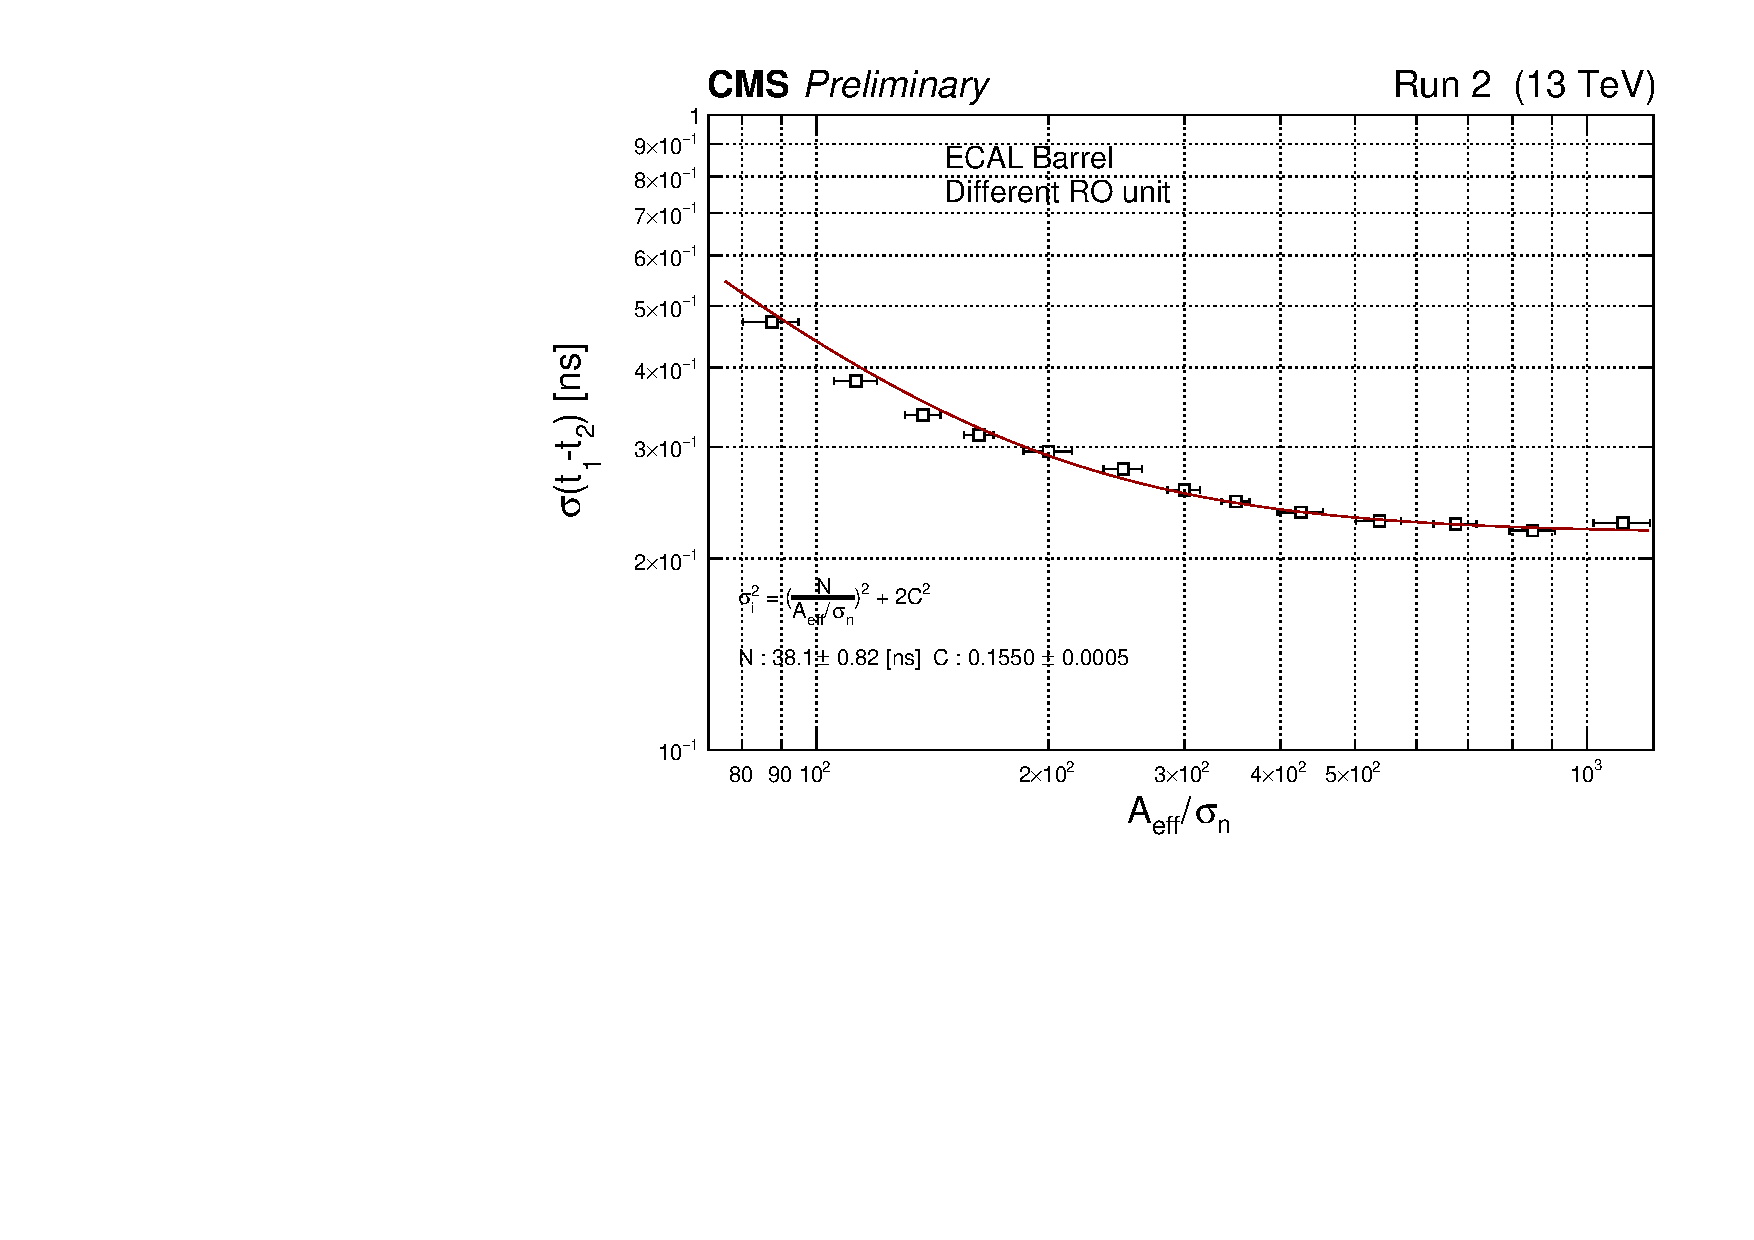
\includegraphics{fig/sec_results/tr_mini_2_locd_gt_01072020101506.pdf}}
%\caption{Different RO unit Resolution for Run 2 }
%\label{2diff}
%\end{center}
%\end{figure}

%\begin{figure}[htbp]
%\begin{center}
%\resizebox{0.48\textwidth}{!}{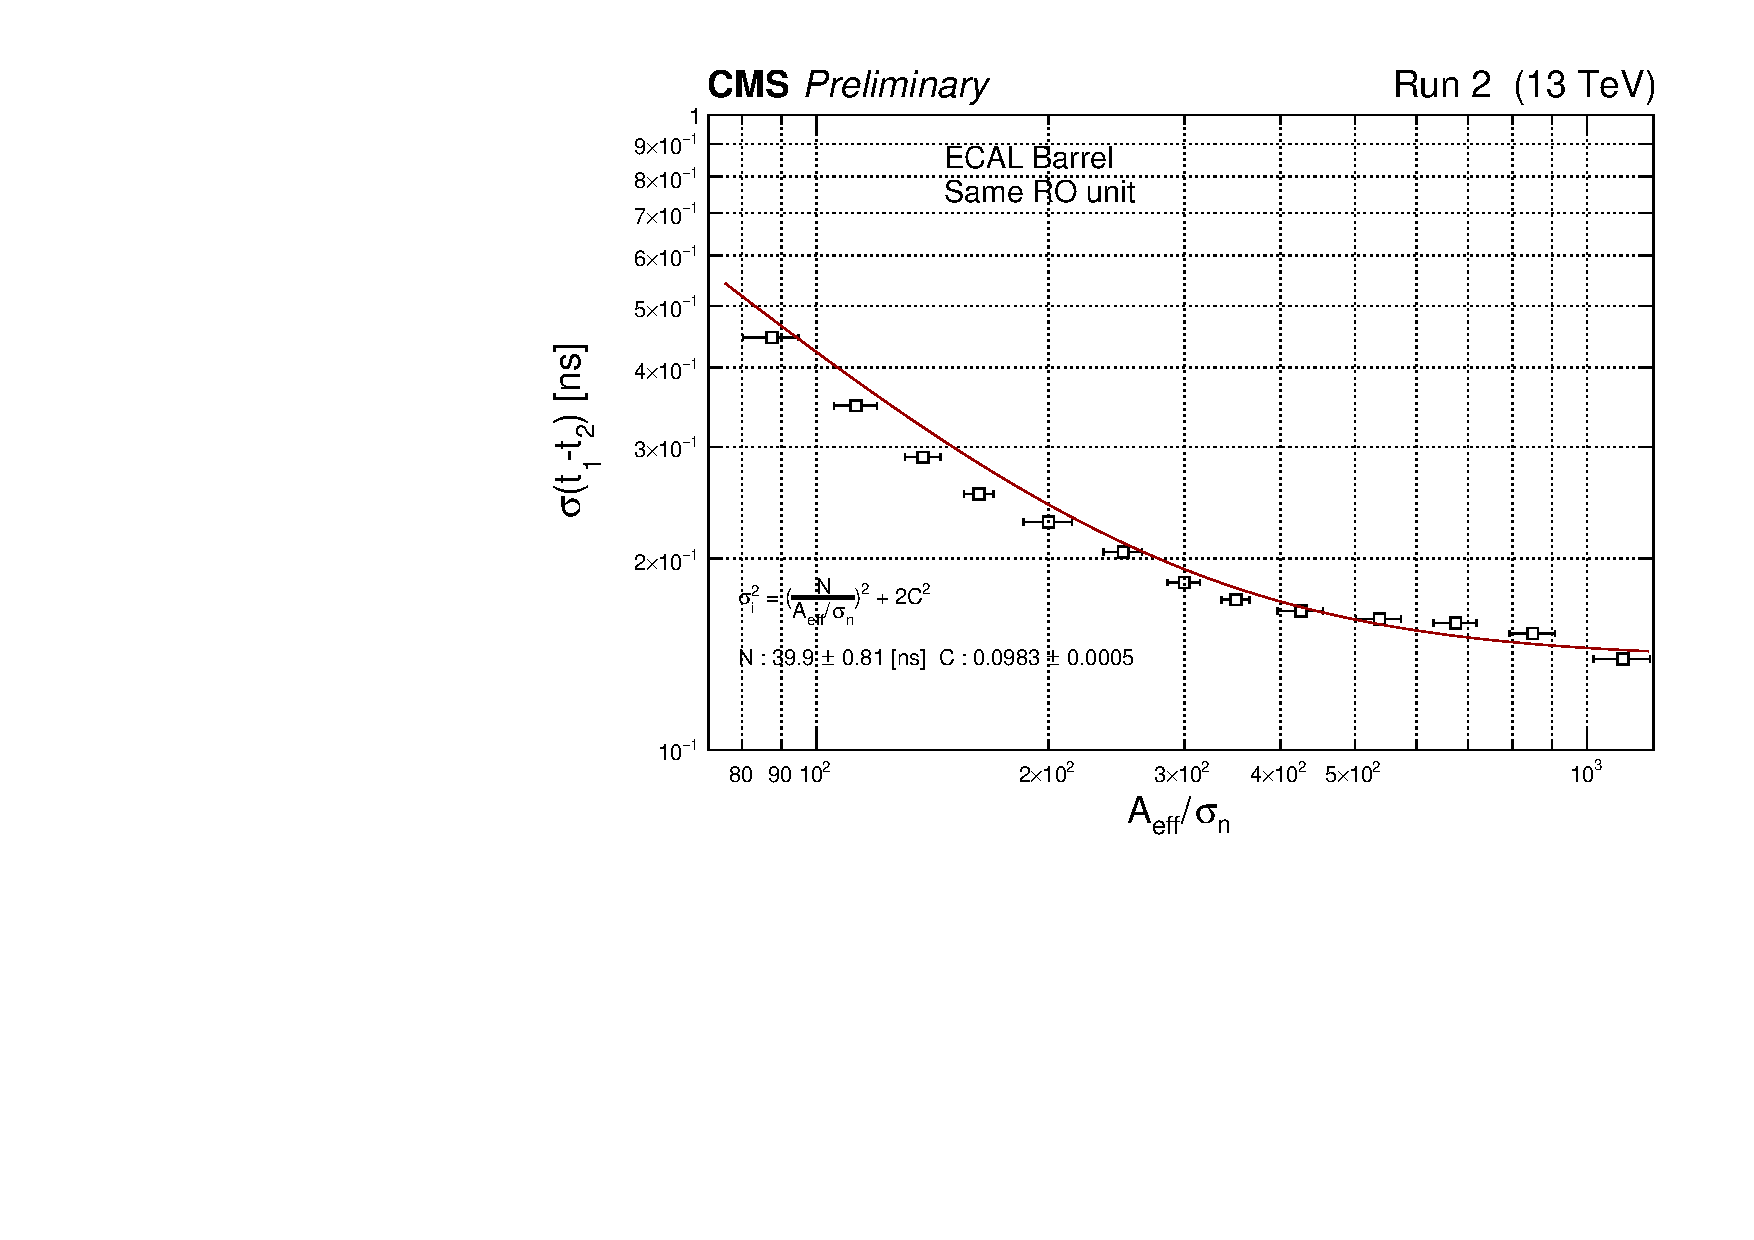
\includegraphics{fig/sec_results/tr_mini_2_loc_gt_01072020101506.pdf}}
%\caption{Same RO unit Resolution for Run 2 }
%\label{2same}
%\end{center}
%\end{figure}

%\begin{figure}[htbp]
%\begin{center}
%\resizebox{0.48\textwidth}{!}{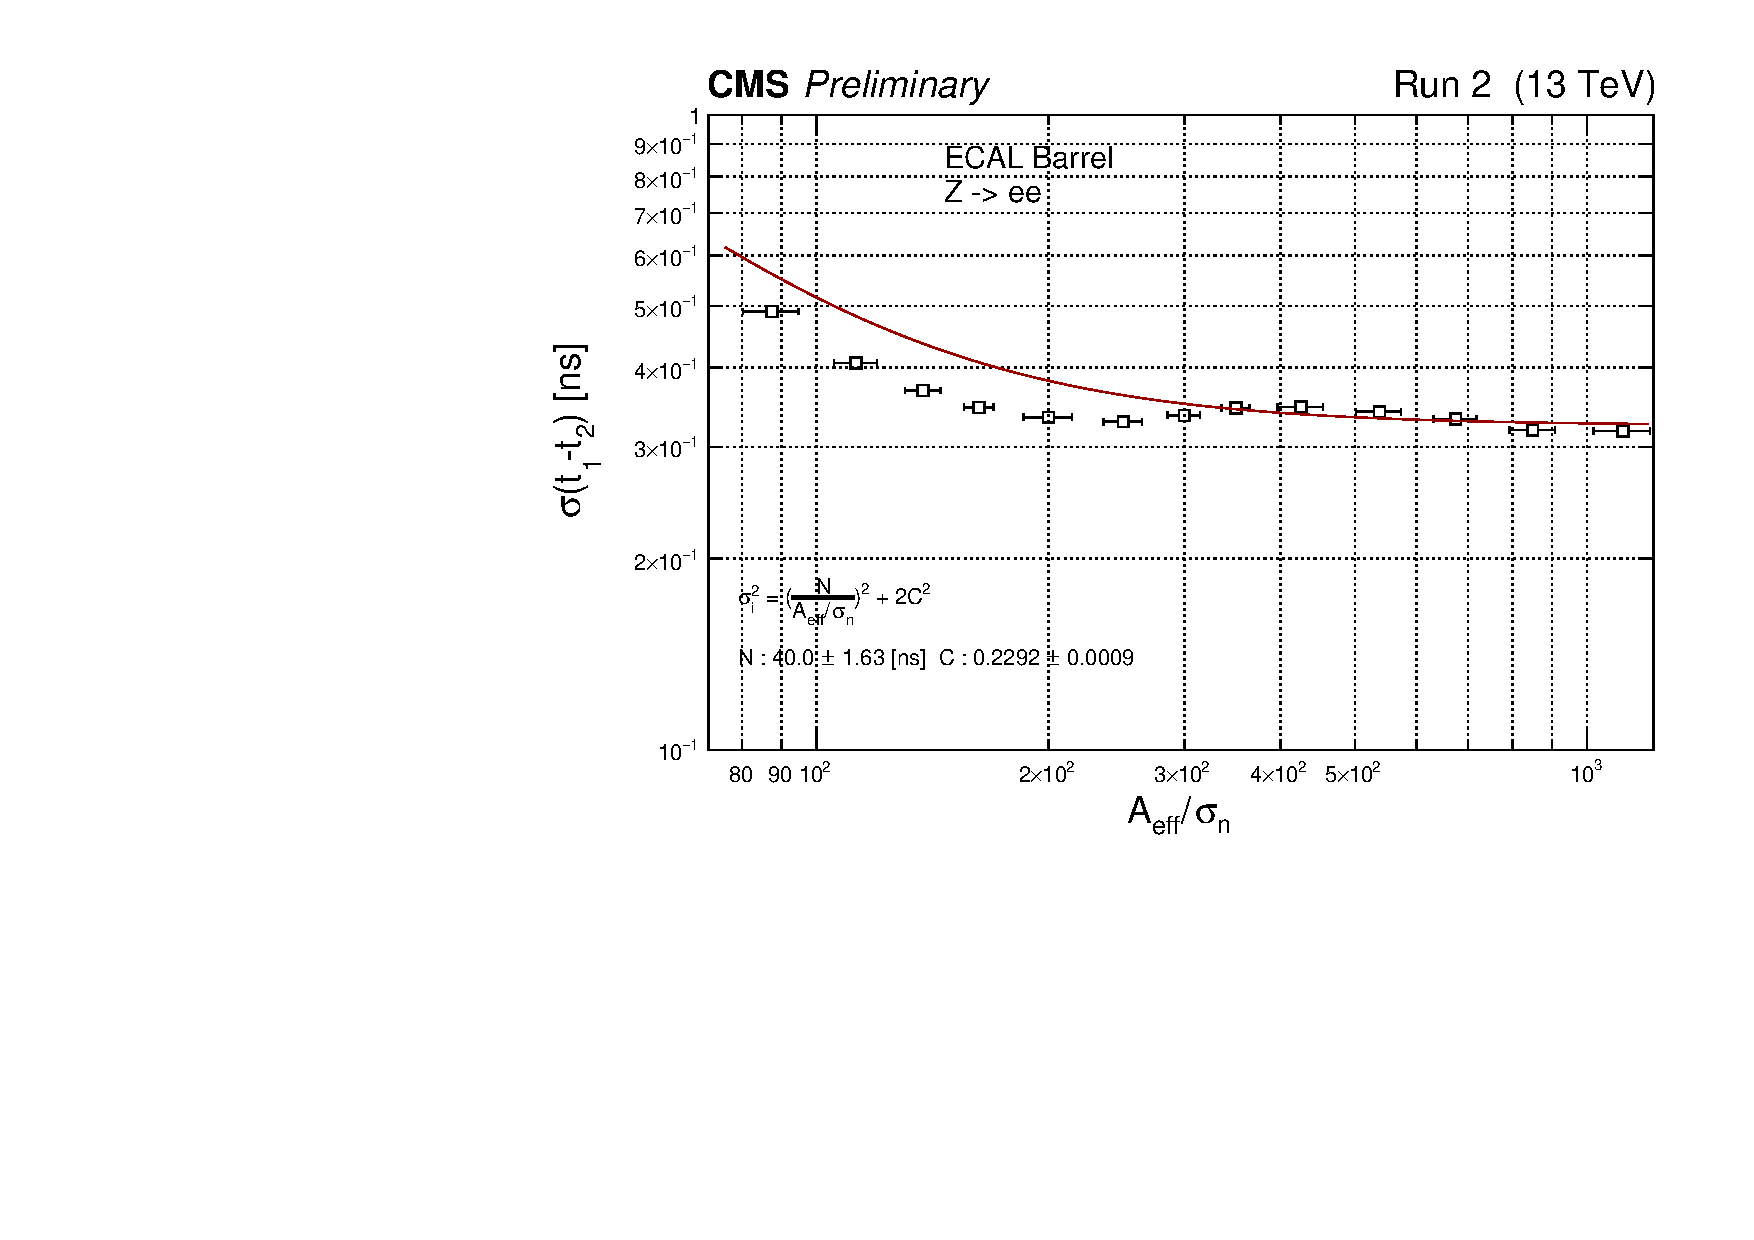
\includegraphics{fig/sec_results/tr_mini_2_glo_gt_01072020101750.pdf}}
%\caption{$Z\rightarrow e^{+}e^{-}$ Resolution for Run 2 }
%\label{2glo}
%\end{center}
%\end{figure}

\begin{figure}[htbp]
\begin{center}
%\resizebox{0.48\textwidth}{!}{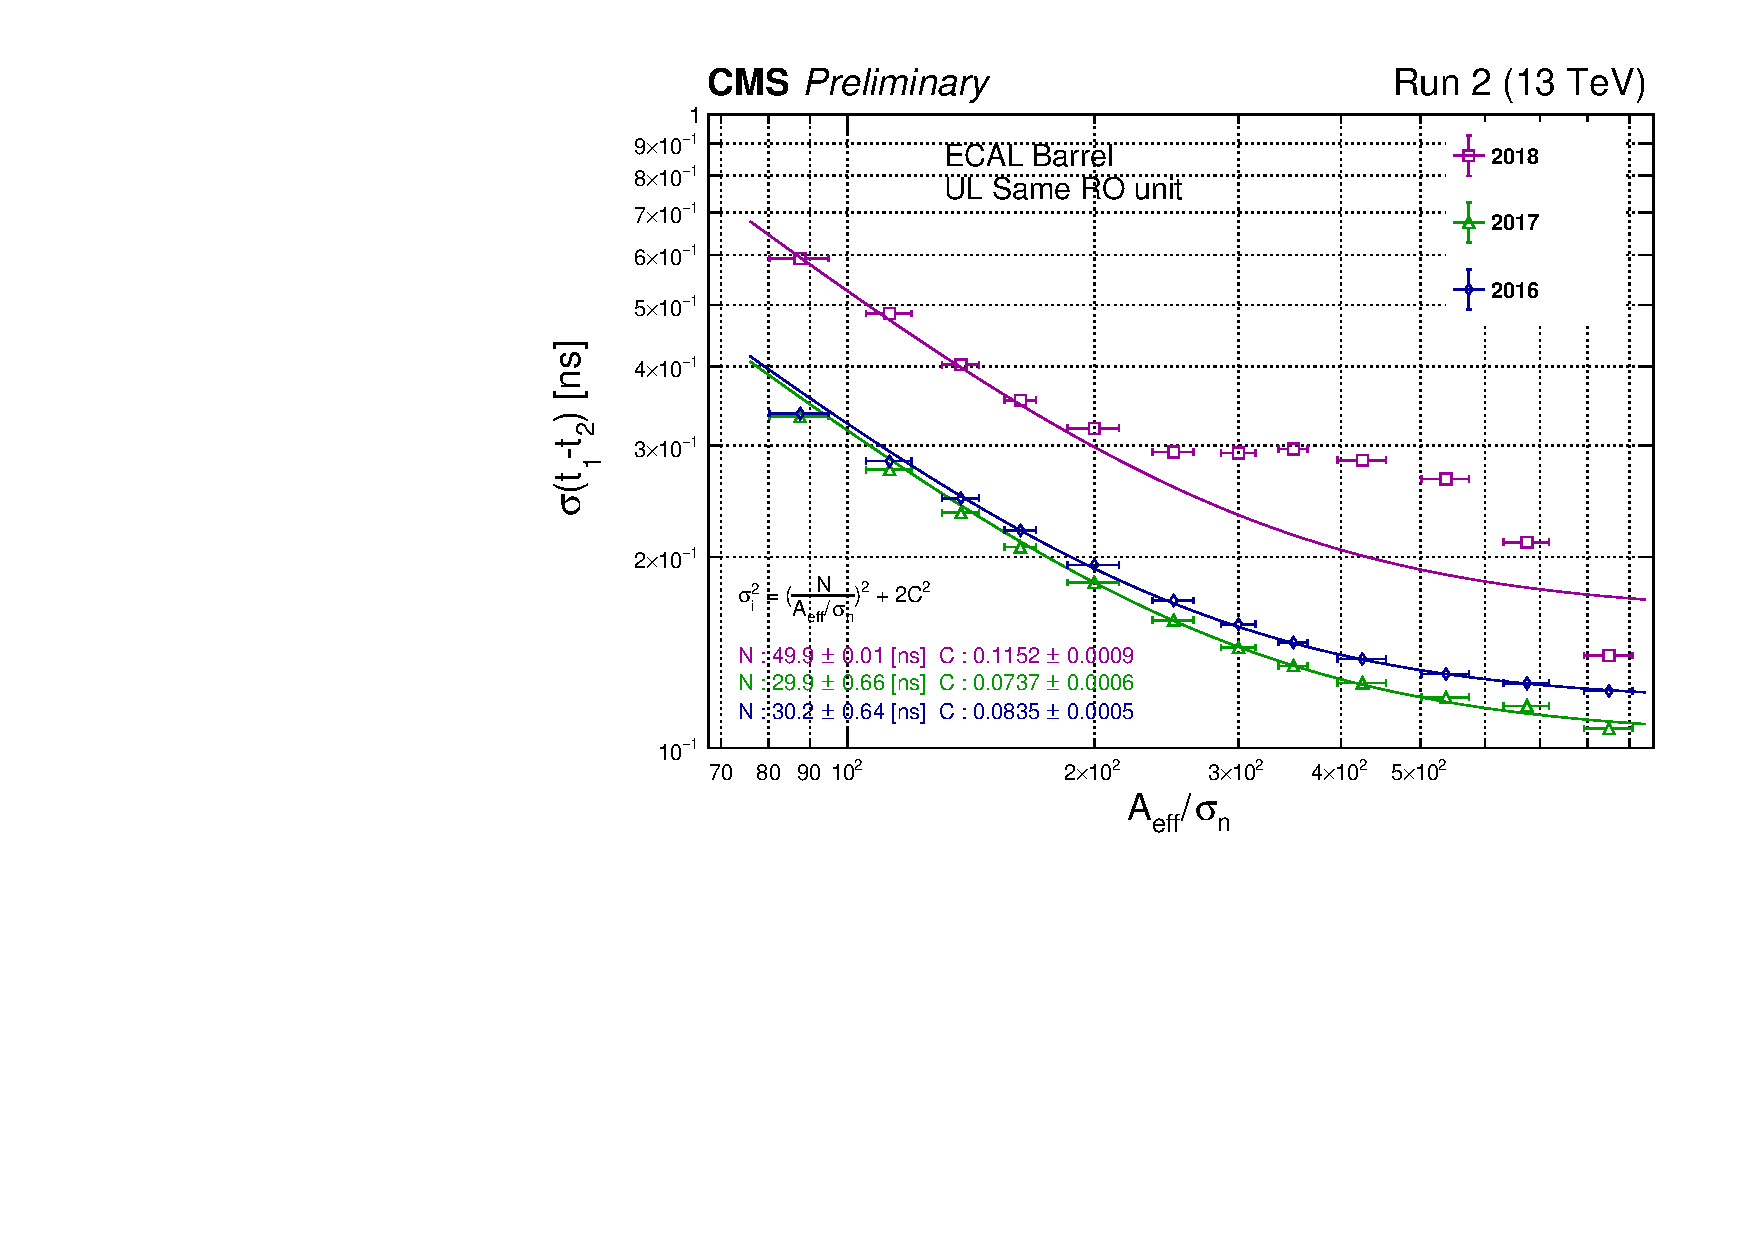
\includegraphics{fig/sec_results/tr_mini_678ul_loc_gt_08082020161532.pdf}}
\resizebox{0.44\textwidth}{!}{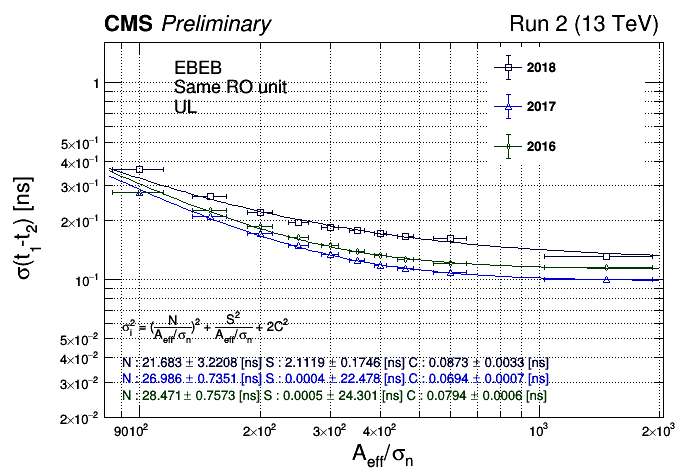
\includegraphics{fig/sec_results/tr_r2_ls_ul_13122021113443.png}}
%\resizebox{0.48\textwidth}{!}{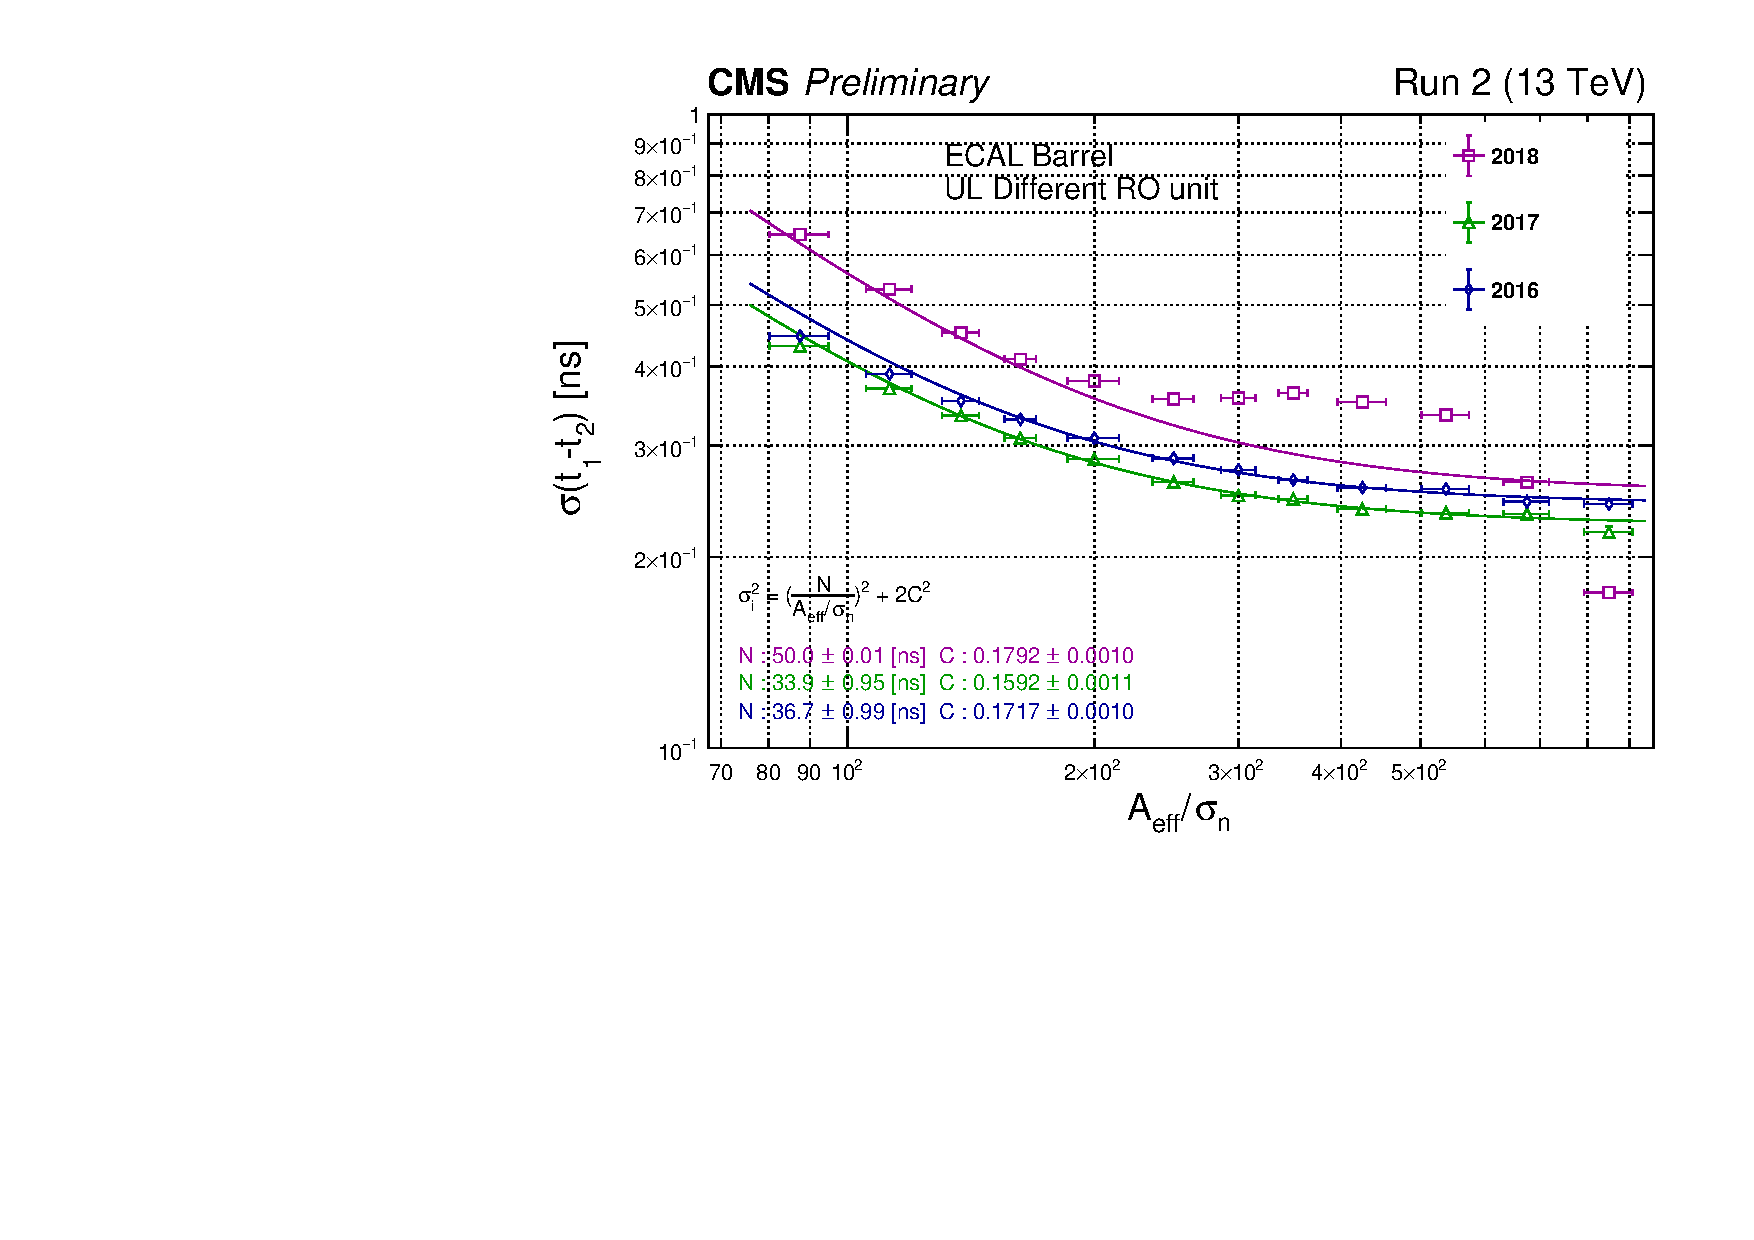
\includegraphics{fig/sec_results/tr_mini_678ul_locd_gt_08082020161532.pdf}}
\resizebox{0.44\textwidth}{!}{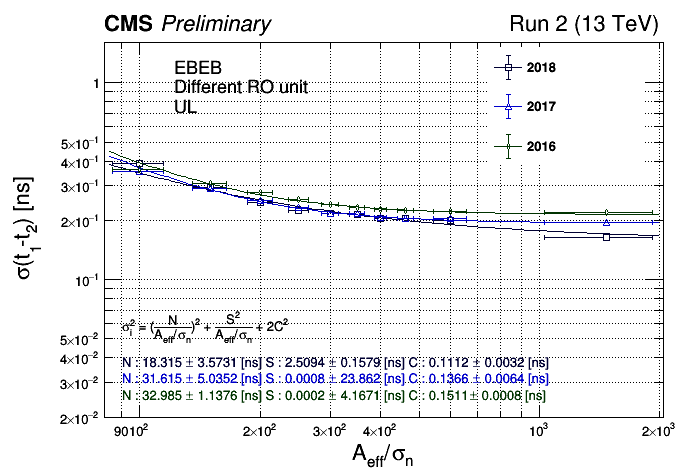
\includegraphics{fig/sec_results/tr_r2_ld_ul_13122021113443.png}}
%\resizebox{0.48\textwidth}{!}{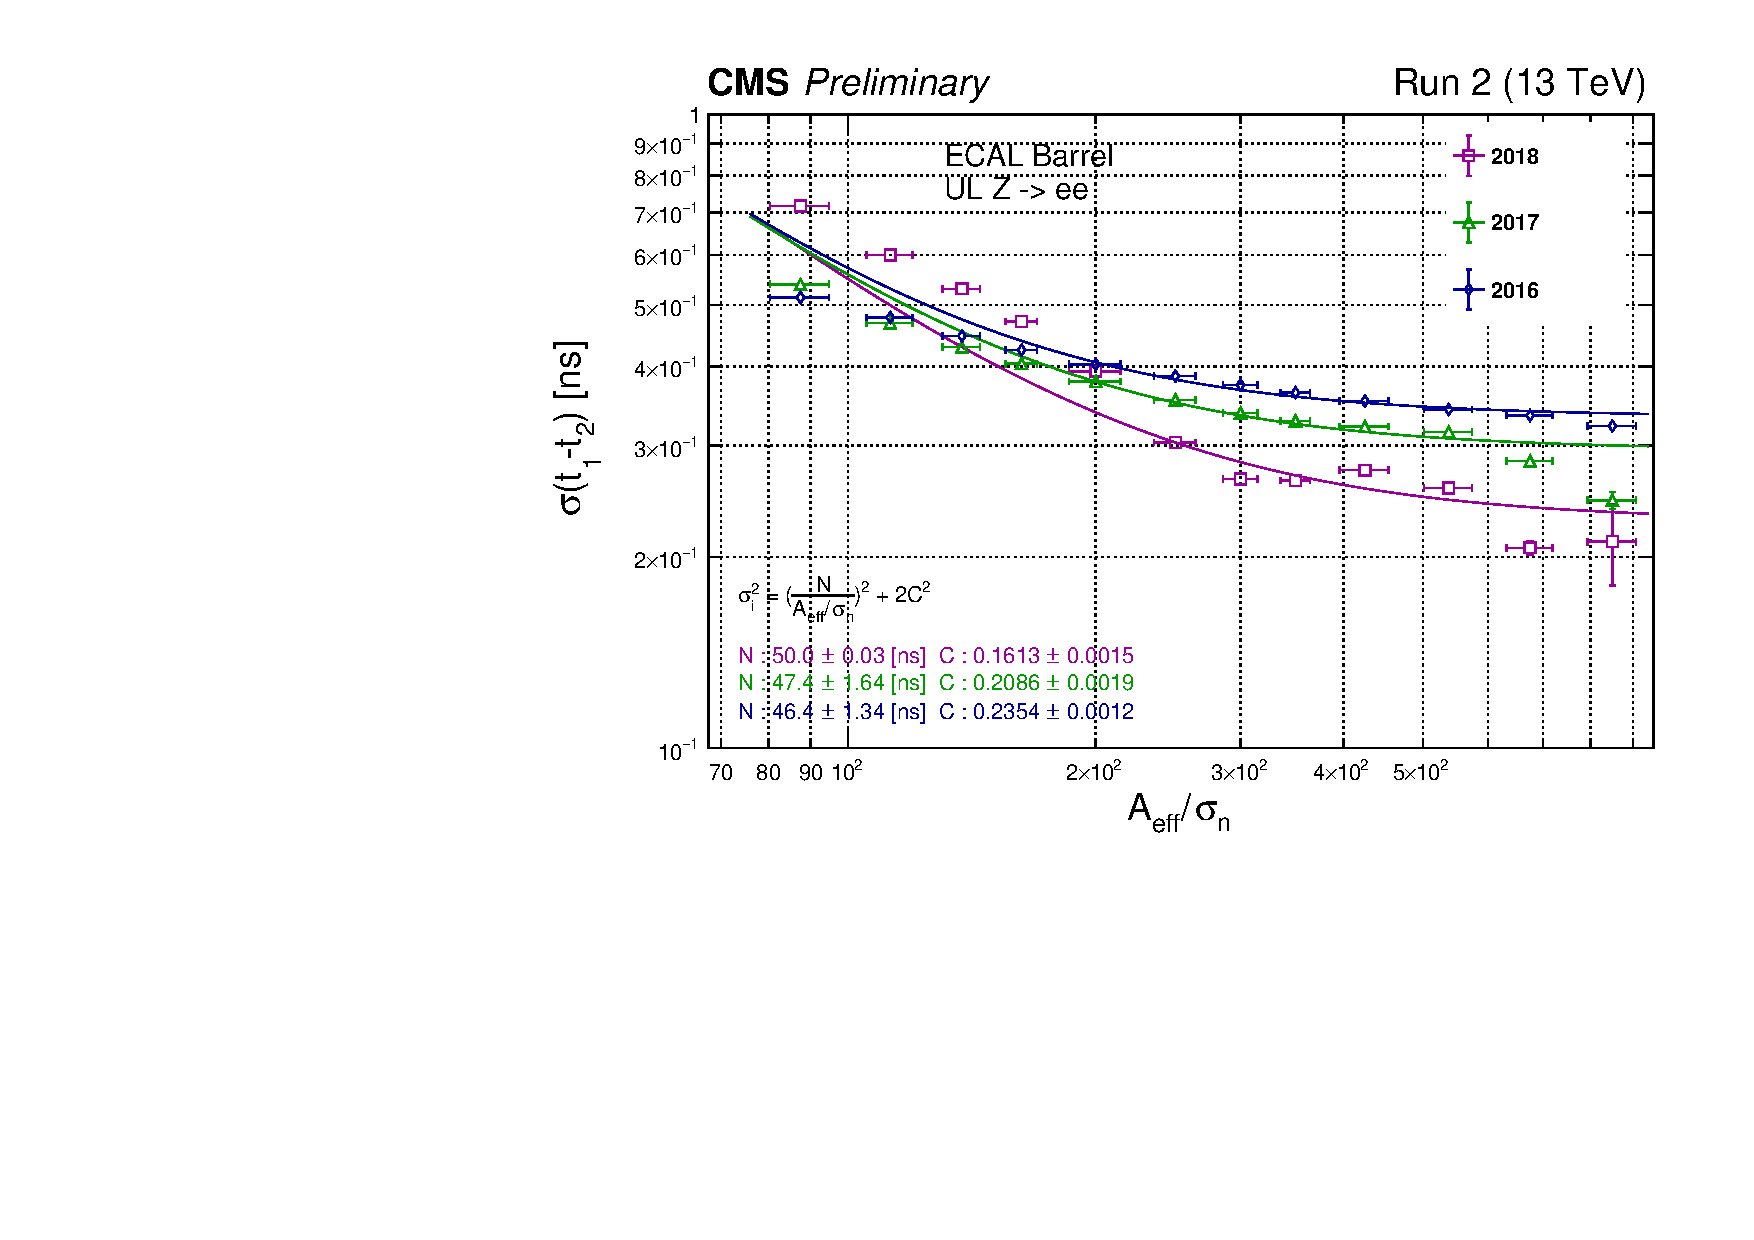
\includegraphics{fig/sec_results/tr_mini_678ul_glo_gt_08082020161532.pdf}}
\resizebox{0.44\textwidth}{!}{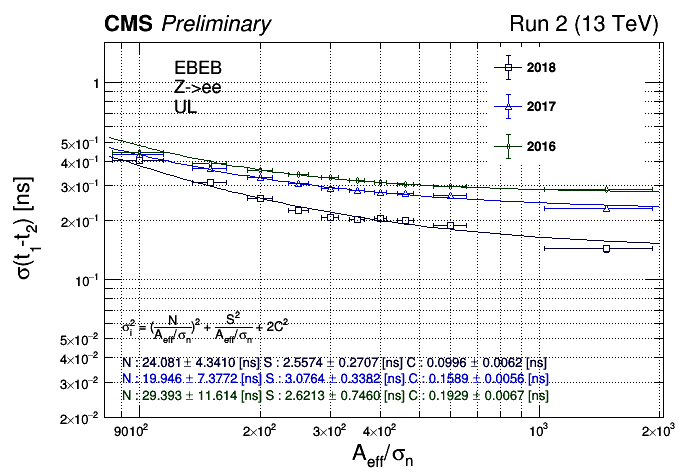
\includegraphics{fig/sec_results/tr_r2_gi_ul_13122021113443.png}}
\caption{
%ECAL time reconstruction resolution for UL Run 2.
ECAL default reconstruction same RO unit, different RO unit, and $Z\rightarrow e^{+}e^{-}$ time resolutions for Ultra Legacy Run 2 produced with the EGamma data-stream for 2018 and Double Egamma data-stream for 2017 and 2016.}
\label{678ULres}
\end{center}
\end{figure}

 The fit parameters for the resolution plots in Figure \ref{678EOYres} and Figure \ref{678ULres} are summarized in the following tables:

%\begin{table}[htbp]
\begin{center}
 \begin{tabular}{ |c|c|c|c| }
 \multicolumn{4}{c}{                            } \\
 \hline
 \multicolumn{4}{|c|}{Same RO Unit}\\
 \hline
 Era & N & S & C \\
 \hline
 \hline
 \multicolumn{4}{|c|}{End of Year}\\
 \hline
 2018 & 0.0023 $\pm$ 66.63 & 2.469 $\pm$ 0.070 & 0.1215 $\pm$ 0.0018 \\
 2017 & 27.107 $\pm$ 0.759 & 0.0003 $\pm$ 16.277 & 0.0693 $\pm$ 0.0007 \\
 2016 & 28.373 $\pm$ 0.765 & 0.0002 $\pm$ 4.6667 & 0.0797 $\pm$ 0.0006 \\
 \hline
 \multicolumn{4}{|c|}{Ultra Legacy}\\
 \hline
 2018 & 21.683 $\pm$ 3.2208 & 2.1119 $\pm$ 0.1746 & 0.0873 $\pm$ 0.0033 \\
 2017 & 26.986 $\pm$ 0.7351 & 0.0004 $\pm$ 22.478 & 0.0694 $\pm$ 0.0007 \\
 2016 & 28.471 $\pm$ 0.7573 & 0.0005 $\pm$ 24.301 & 0.0794 $\pm$ 0.0006 \\
 \hline
 \end{tabular}
\end{center}
%\end{table}
 
%\begin{table}[htbp]
 \begin{center}
 \begin{tabular}{ |c|c|c|c| }
 \multicolumn{4}{c}{                            } \\
 \hline
  \multicolumn{4}{|c|}{Different RO Unit}\\
 \hline
 Era & N & S & C \\
 \hline
 \multicolumn{4}{|c|}{End of Year}\\
 \hline
 2018 & 0.0039 $\pm$ 21.491 & 2.5813 $\pm$ 0.0739 & 0.1380 $\pm$ 0.0018 \\
 2017 & 31.152 $\pm$ 4.2954 & 0.0016 $\pm$ 20.231 & 0.1370 $\pm$ 0.0068 \\
 2016 & 32.840 $\pm$ 1.1229 & 0.0002 $\pm$ 3.6374 & 0.1521 $\pm$ 0.0008 \\
 \hline
 \multicolumn{4}{|c|}{Ultra Legacy}\\
 \hline
 2018 & 18.315 $\pm$ 3.5731 & 2.5094 $\pm$ 0.1579 & 0.1122 $\pm$ 0.0032 \\
 2017 & 31.615 $\pm$ 5.0352 & 0.0008 $\pm$ 23.862 & 0.1366 $\pm$ 0.0064 \\
 2016 & 32.985 $\pm$ 1.1376 & 0.0002 $\pm$ 4.1671 & 0.1511 $\pm$ 0.0008 \\
 \hline
\end{tabular}
\end{center}
%\end{table}

%\begin{table}[htbp]
\begin{center}
 \begin{tabular}{ |c|c|c|c| }
 \multicolumn{4}{c}{                            } \\
 \hline
  \multicolumn{4}{|c|}{$Z\rightarrow e^{+}e^{-}$}\\
 \hline
 Era & N & S & C \\
 \hline
 \multicolumn{4}{|c|}{End of Year}\\
 \hline
 2018 & 31.560 $\pm$ 5.3817 & 1.2827 $\pm$ 0.3950 & 0.1558 $\pm$ 0.0012 \\
 2017 & 20.250 $\pm$ 7.1382 & 3.0328 $\pm$ 0.3376 & 0.1599 $\pm$ 0.0055 \\
 2016 & 34.297 $\pm$ 10.641 & 2.1725 $\pm$ 0.9142 & 0.1980 $\pm$ 0.0064 \\
 \hline
 \multicolumn{4}{|c|}{Ultra Legacy}\\
 \hline
 2018 & 24.081 $\pm$ 4.3410 & 2.5574 $\pm$ 0.2707 & 0.0996 $\pm$ 0.0062 \\
 2017 & 19.946 $\pm$ 7.3772 & 3.0764 $\pm$ 0.3382 & 0.1589 $\pm$ 0.0056 \\
 2016 & 29.393 $\pm$ 11.614 & 2.6213 $\pm$ 0.7460 & 0.1929 $\pm$ 0.0057 \\
\hline
\end{tabular}
\end{center}
%\end{table}

%\begin{figure}[htbp]
%\begin{center}
%\resizebox{0.48\textwidth}{!}{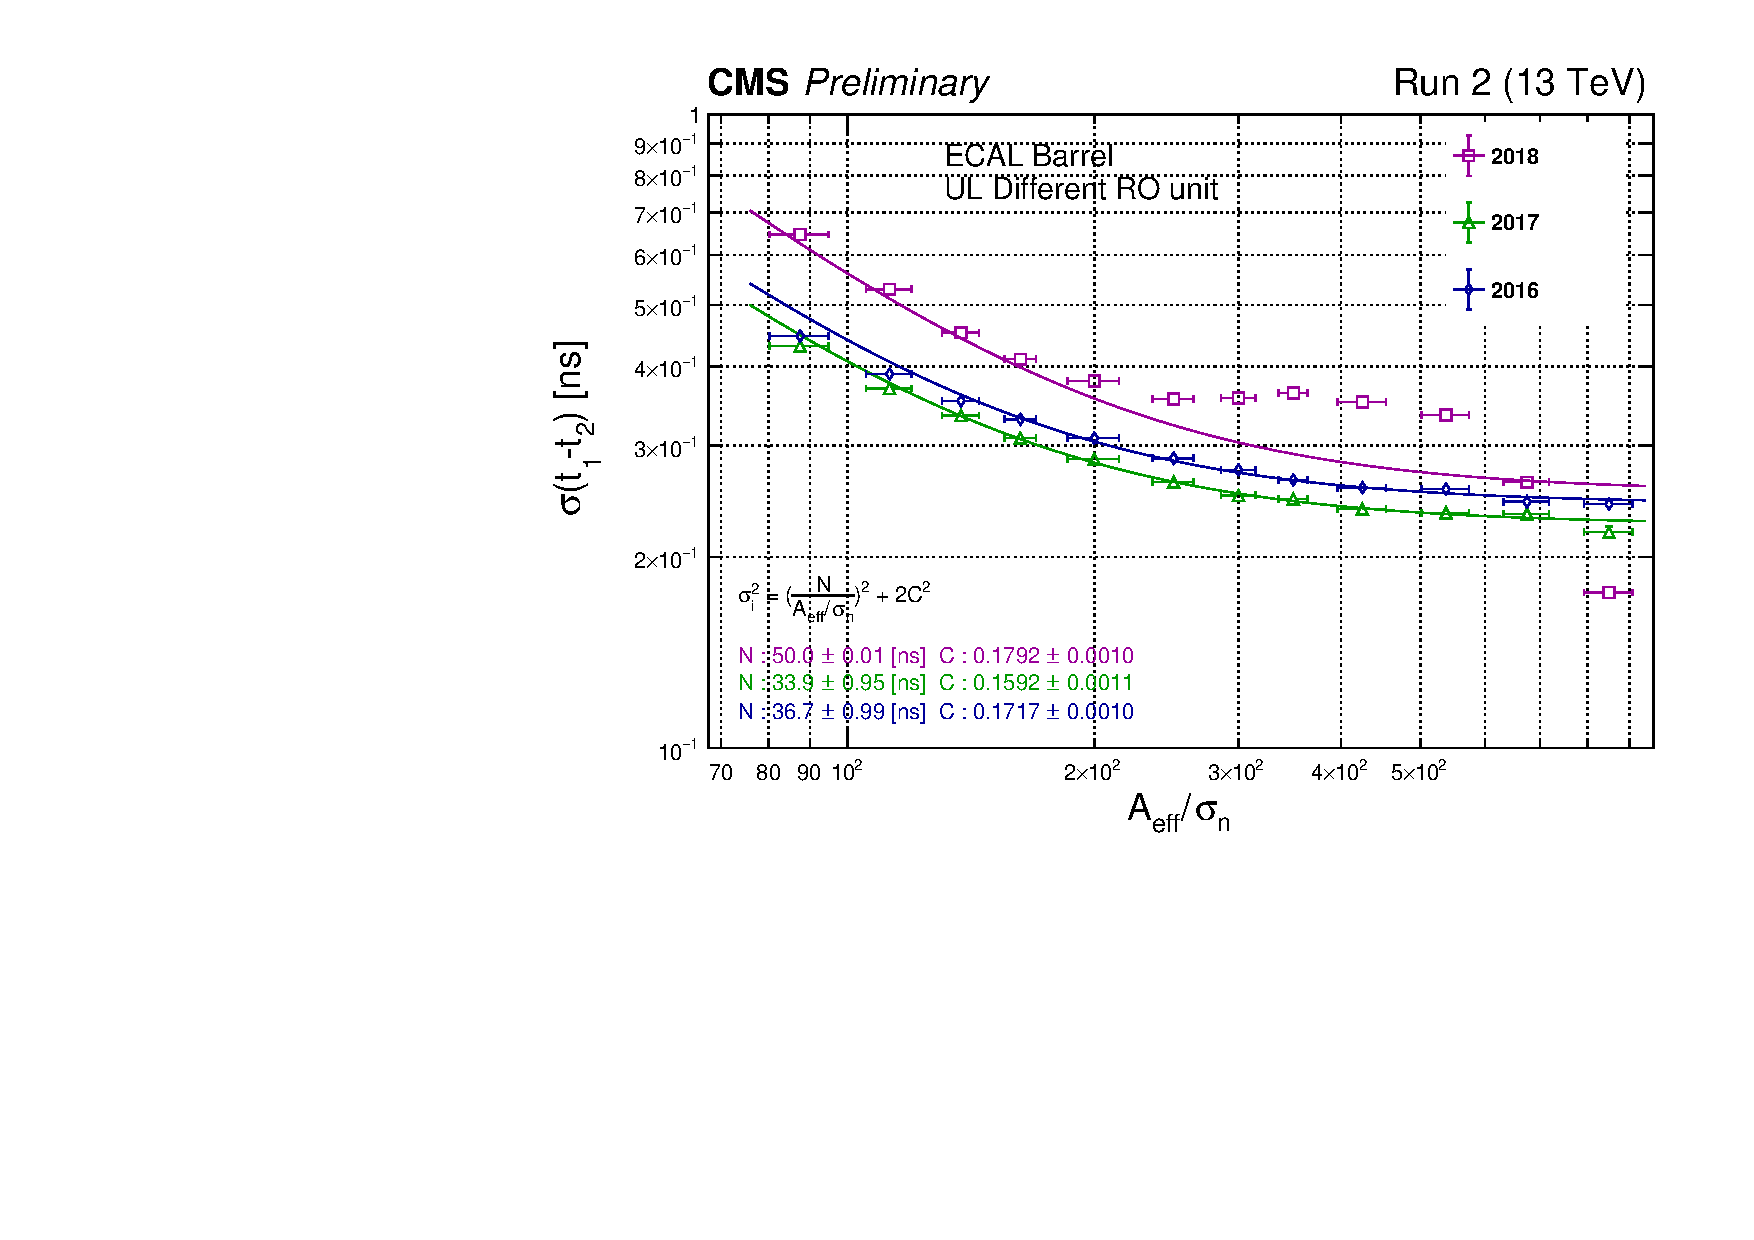
\includegraphics{fig/sec_results/tr_mini_678ul_locd_gt_08082020161532.pdf}}
%\caption{Different RO unit Resolution for Run 2 UL}
%\label{678ULld}
%\end{center}
%\end{figure}

%\begin{figure}[htbp]
%\begin{center}
%\resizebox{0.48\textwidth}{!}{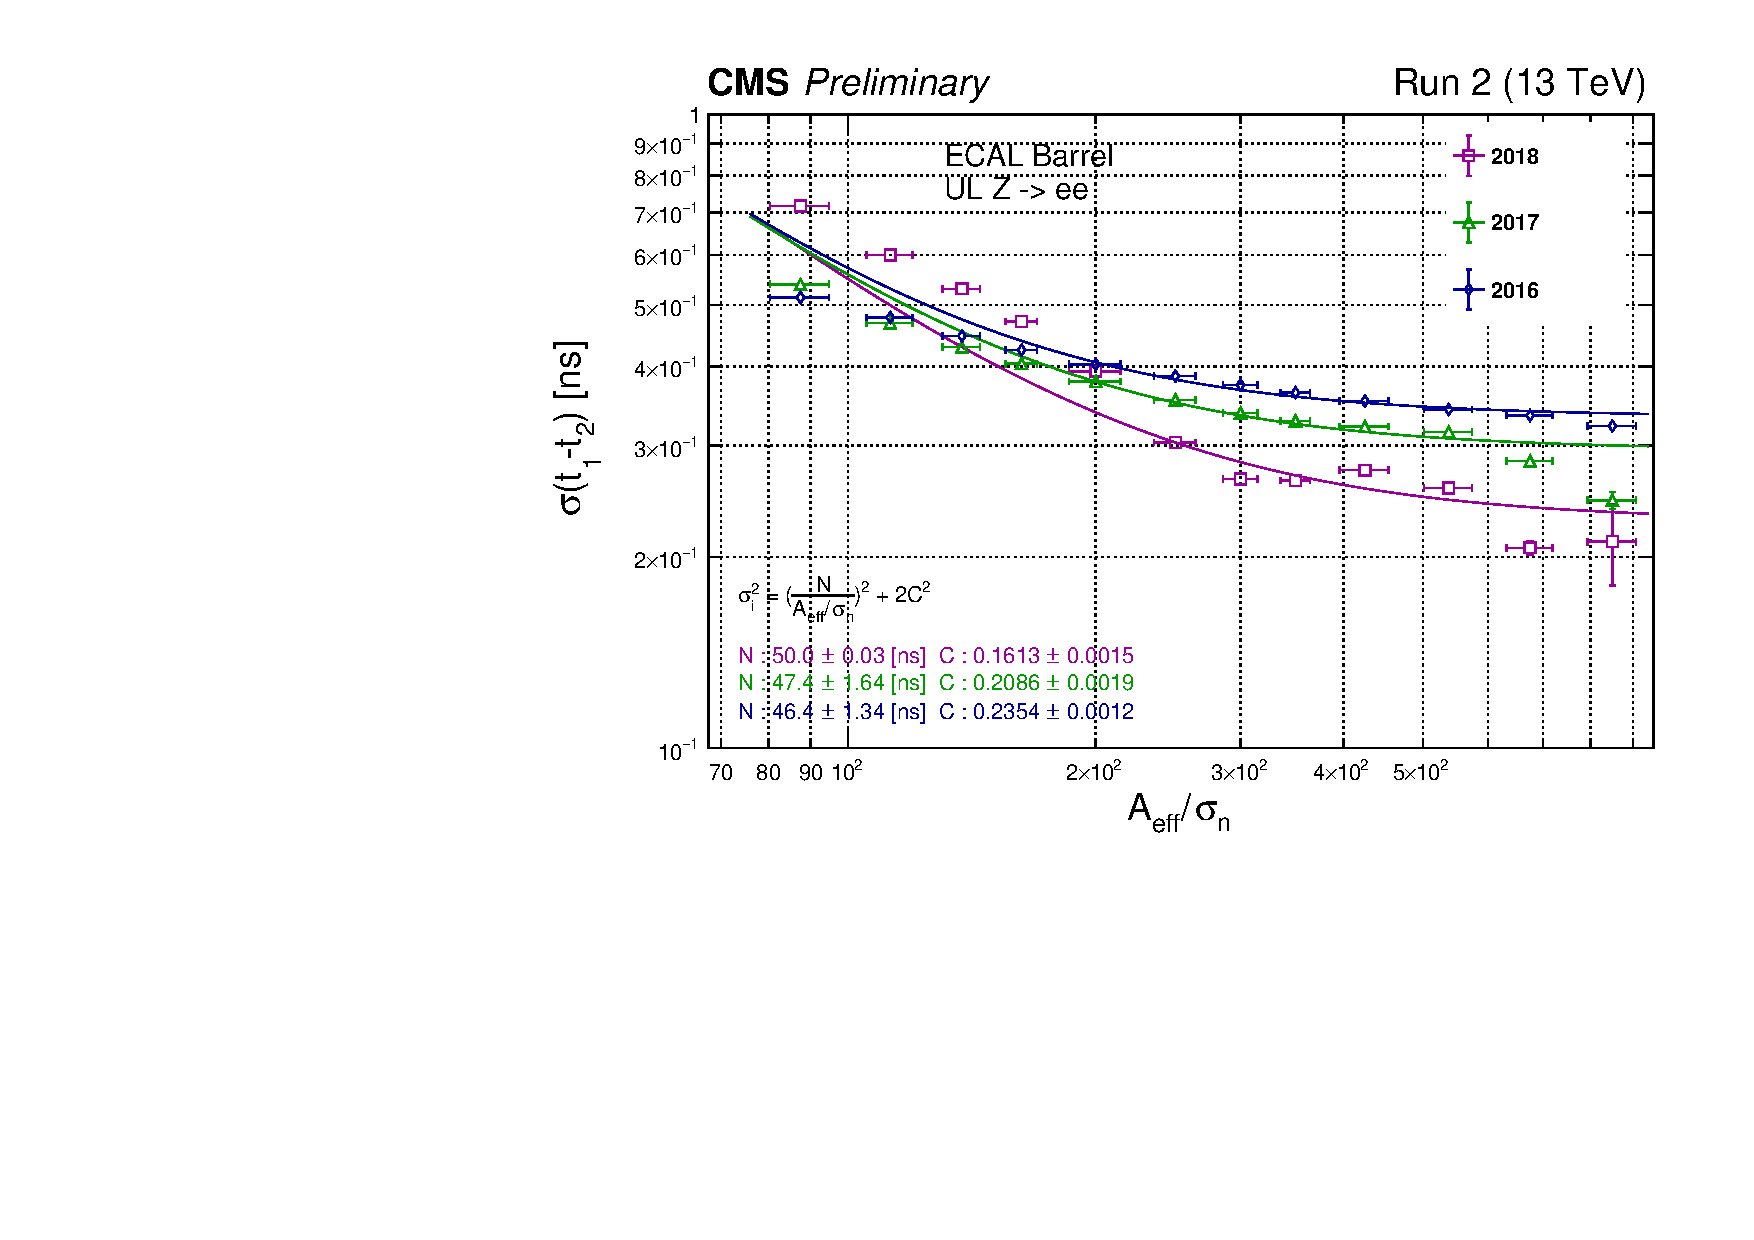
\includegraphics{fig/sec_results/tr_mini_678ul_glo_gt_08082020161532.pdf}}
%\caption{$Z\rightarrow e^{+}e^{-}$ Resolution for Run 2 UL}
%\label{678ULglo}
%\end{center}
%\end{figure}

%\begin{figure}[htbp]
%\begin{center}
%\resizebox{0.48\textwidth}{!}{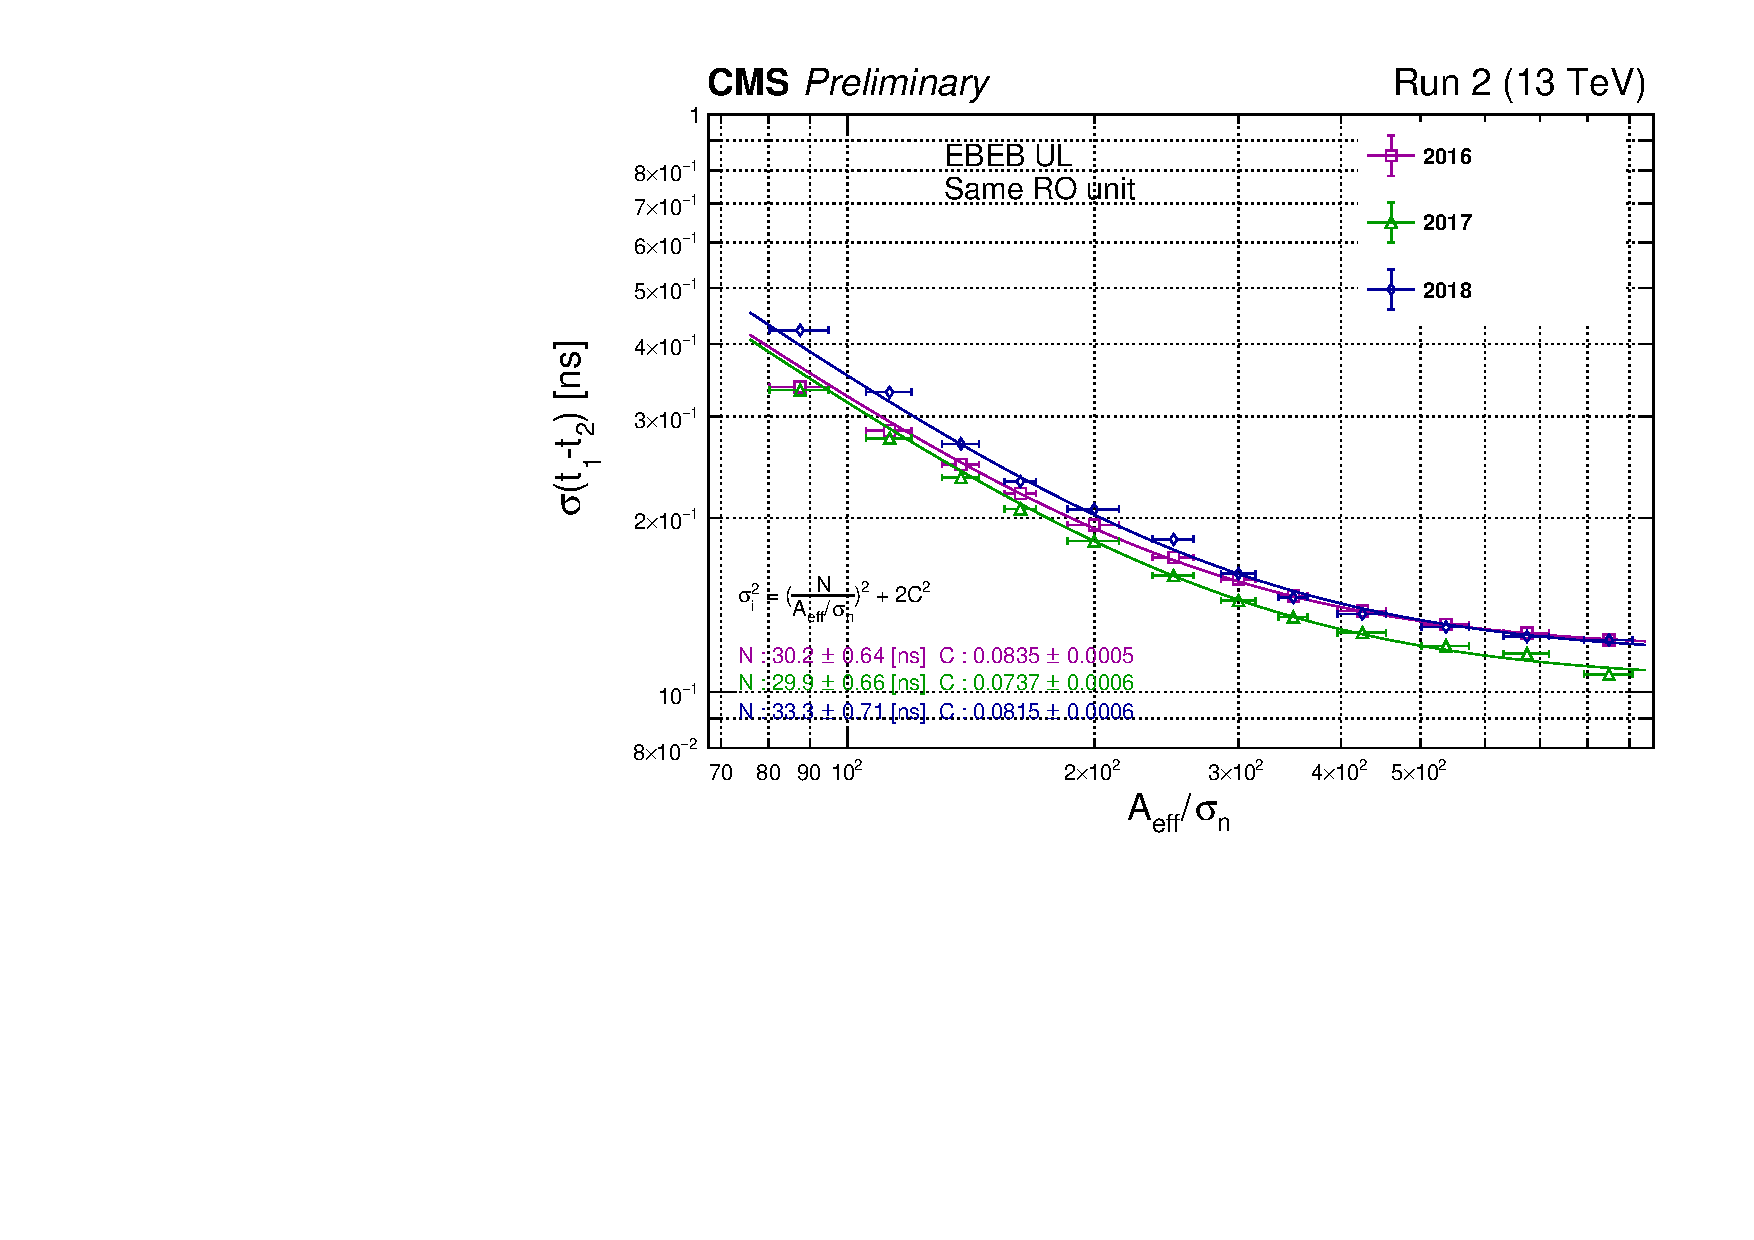
\includegraphics{fig/sec_results/tr_mini_678ul_ls_18gt28_21102020113501.pdf}}
%\caption{Same RO Resolution for Run 2 UL GT 28}
%\label{678UL28ls}
%\end{center}
%\end{figure}

%\begin{figure}[htbp]
%\begin{center}
%\resizebox{0.48\textwidth}{!}{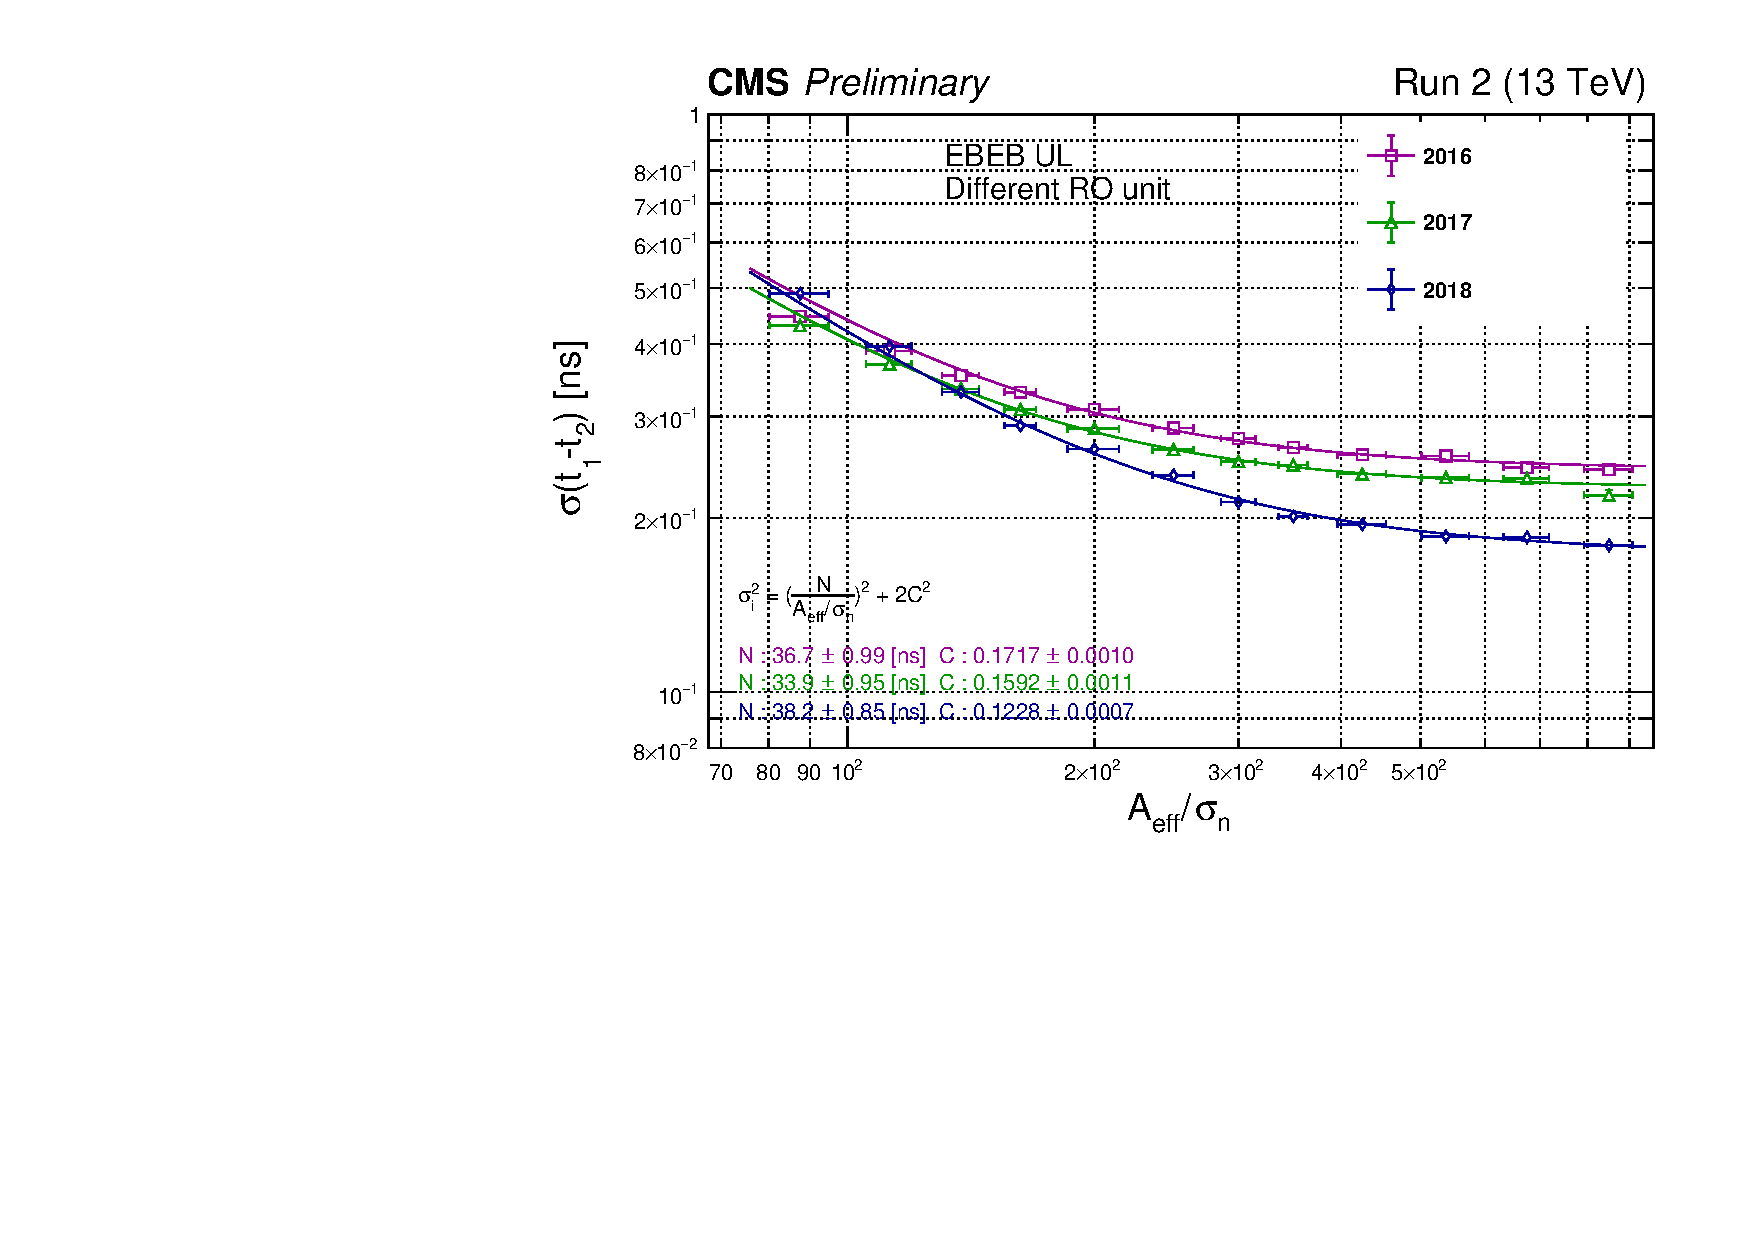
\includegraphics{fig/sec_results/tr_mini_678ul_ld_18gt28_21102020113501.pdf}}
%\caption{Different RO Resolution for Run 2 UL Gt 28}
%\label{678UL28ld}
%\end{center}
%\end{figure}

%\begin{figure}[htbp]
%\begin{center}
%\resizebox{0.48\textwidth}{!}{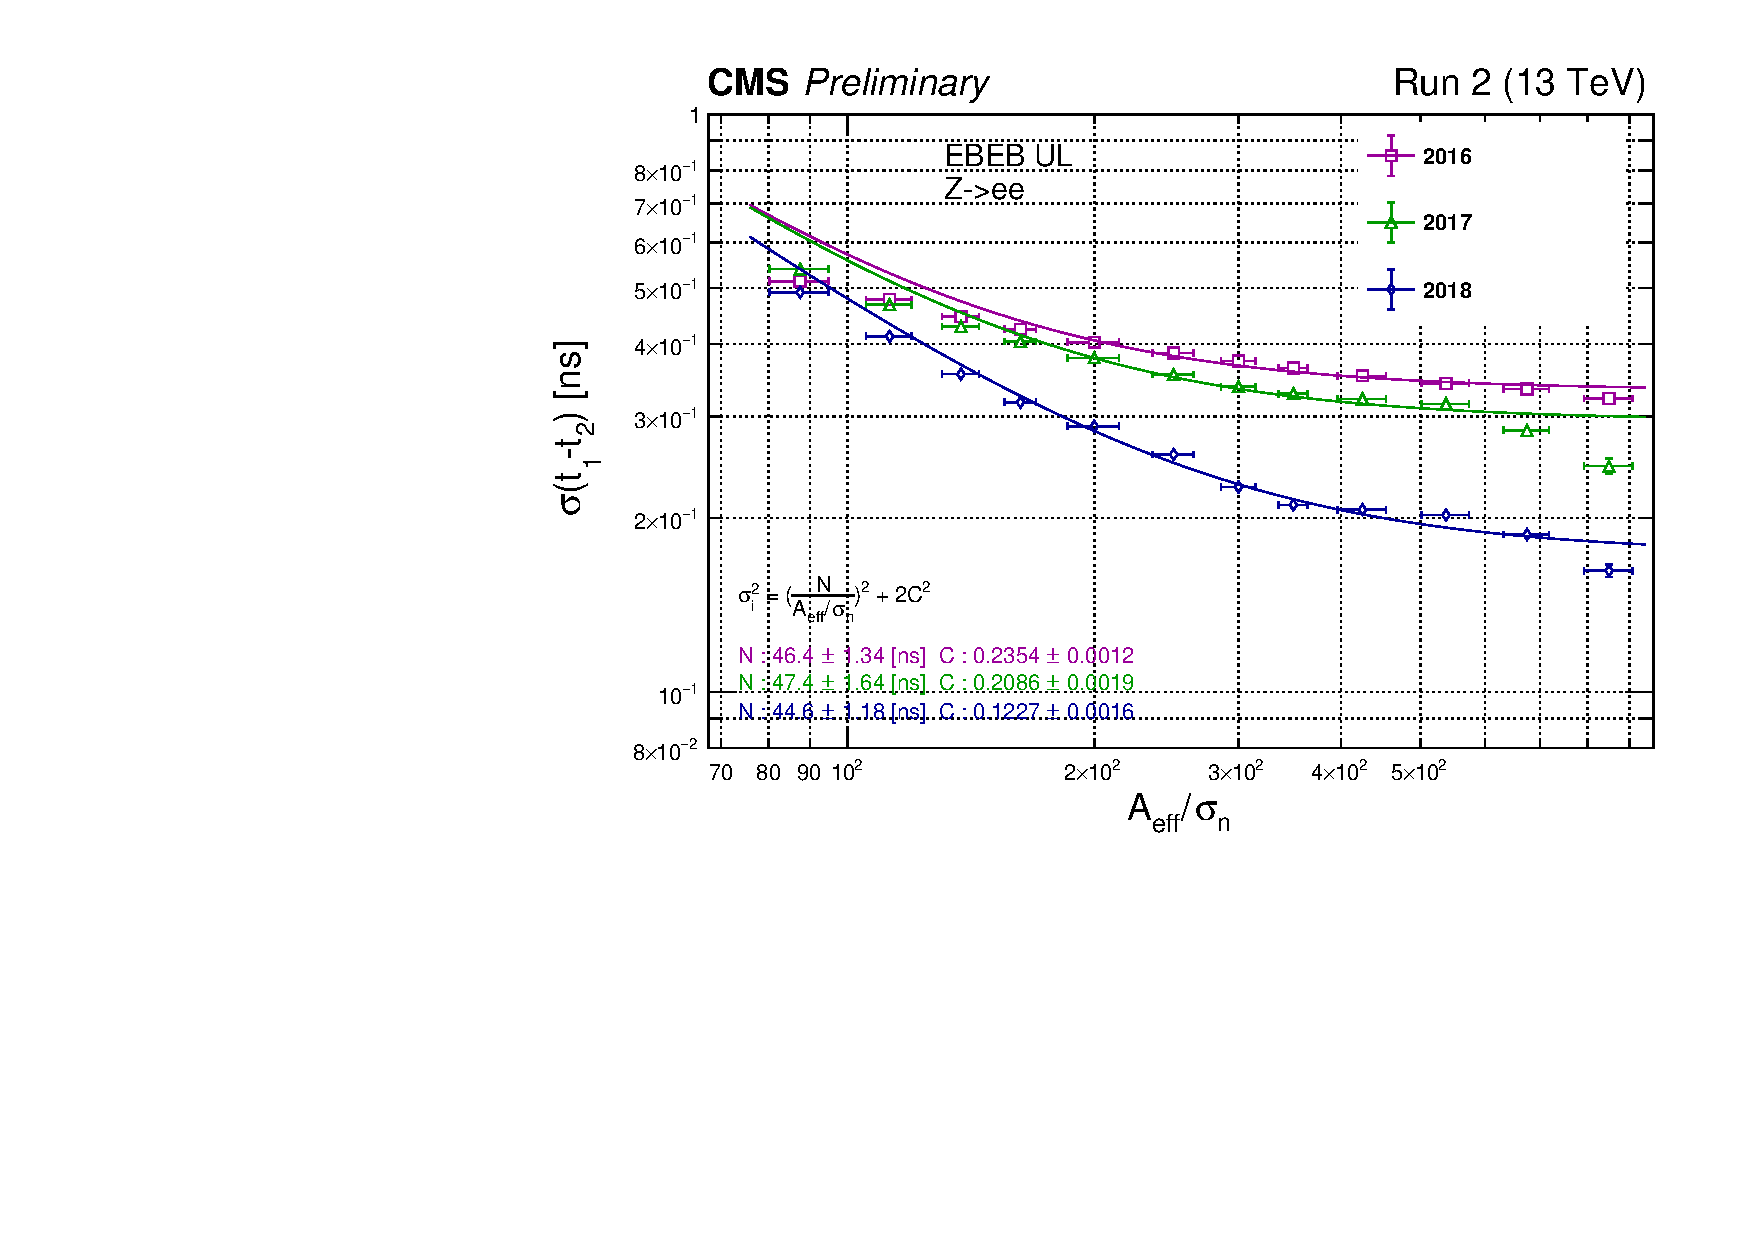
\includegraphics{fig/sec_results/tr_mini_678ul_gi_18gt28_21102020113501.pdf}}
%\caption{$Z\rightarrow e^{+}e^{-}$ Resolution for Run 2 UL GT 28}
%\label{678UL28glo}
%\end{center}
%\end{figure}

%\FloatBarrier
%\subsection{Comparison of Proposed Timing Algorithms}
%In the following section the time resolutions achieved by each method is compared the resolution achieved by the ratio method.  

Results for the KUCC method with the Run 2 EOY data streams where produced for 2018 with CMSSW 11.3.0 pre6 using GT 112X\_dataRun3\_Prompt\_v2. For 2016 and 2017 the results where produced with CMSSW 9.4.10 using GT 94X\_dataRun2\_v10 for all eras of 2016 and GT 94X\_dataRun2\_v11 for all eras of 2017. While characterizing the cross correlation method across all eras in Run 2 would be preferable, due to the limited availability of RAW data streams only selected portions of the eras where available to produce resolutions for each data stream are shown in the following table.

\begin{center}
 \begin{tabular}{ |l|c| }
 \hline
 MINIAOD Data Stream & Percent Processed \\ 
 \hline
 \multicolumn{2}{|c|}{EGamma Run 2018 EOY }\\
 \hline
 Run2018A-17Sep2018-v2 & 95\%\\
 Run2018B-17Sep2018-v1 & 16\%\\
 Run2018C-17Sep2018-v1 & 8\%\\
 Run2018D-22Jan2019-v2 & 94\%\\
 \hline
 \multicolumn{2}{|c|}{DoubleEG Run 2017 EOY }\\
 \hline
 Run2017B-31Mar2018-v1 & 6\%\\
 Run2017C-31Mar2018-v1 & 3\%\\
 \hline
 \multicolumn{2}{|c|}{Double EG Run 2016 EOY }\\
 \hline
 Run2016B-17Jul2018\_ver2-v1 & 83\%\\
 Run2016E-17Jul2018-v1 & 16\%\\
 Run2016F-17Jul2018-v1 & 12\%\\
 \hline
 \end{tabular}
\end{center}

%The fit for the resolution plots using the KUCC method is extended by the addition of the stochastic term as follows:
%\begin{equation}
%    \sigma^{2}_{i} = (\frac{N}{A_{eff}/\sigma_{N}})^{2} + \frac{S^{2}}{A_{eff}/\sigma_{N}} + 2C^{2}\\
%    \label{eq_ccres}
%\end{equation}
%Previously the precision of the resolution plots was insufficient to constrain the stochastic term and was therefore not included in the fit.

Resolution plots where produced both the KUCC method, in Figure \ref{678CCres}, and the ratio method for comparison, in Figure \ref{678e5Ratiores}, with the these data streams. The fit parameters for the resolution plots are summarized in the following tables.

\begin{figure}[htbp]
\begin{center}
%\resizebox{0.32\textwidth}{!}{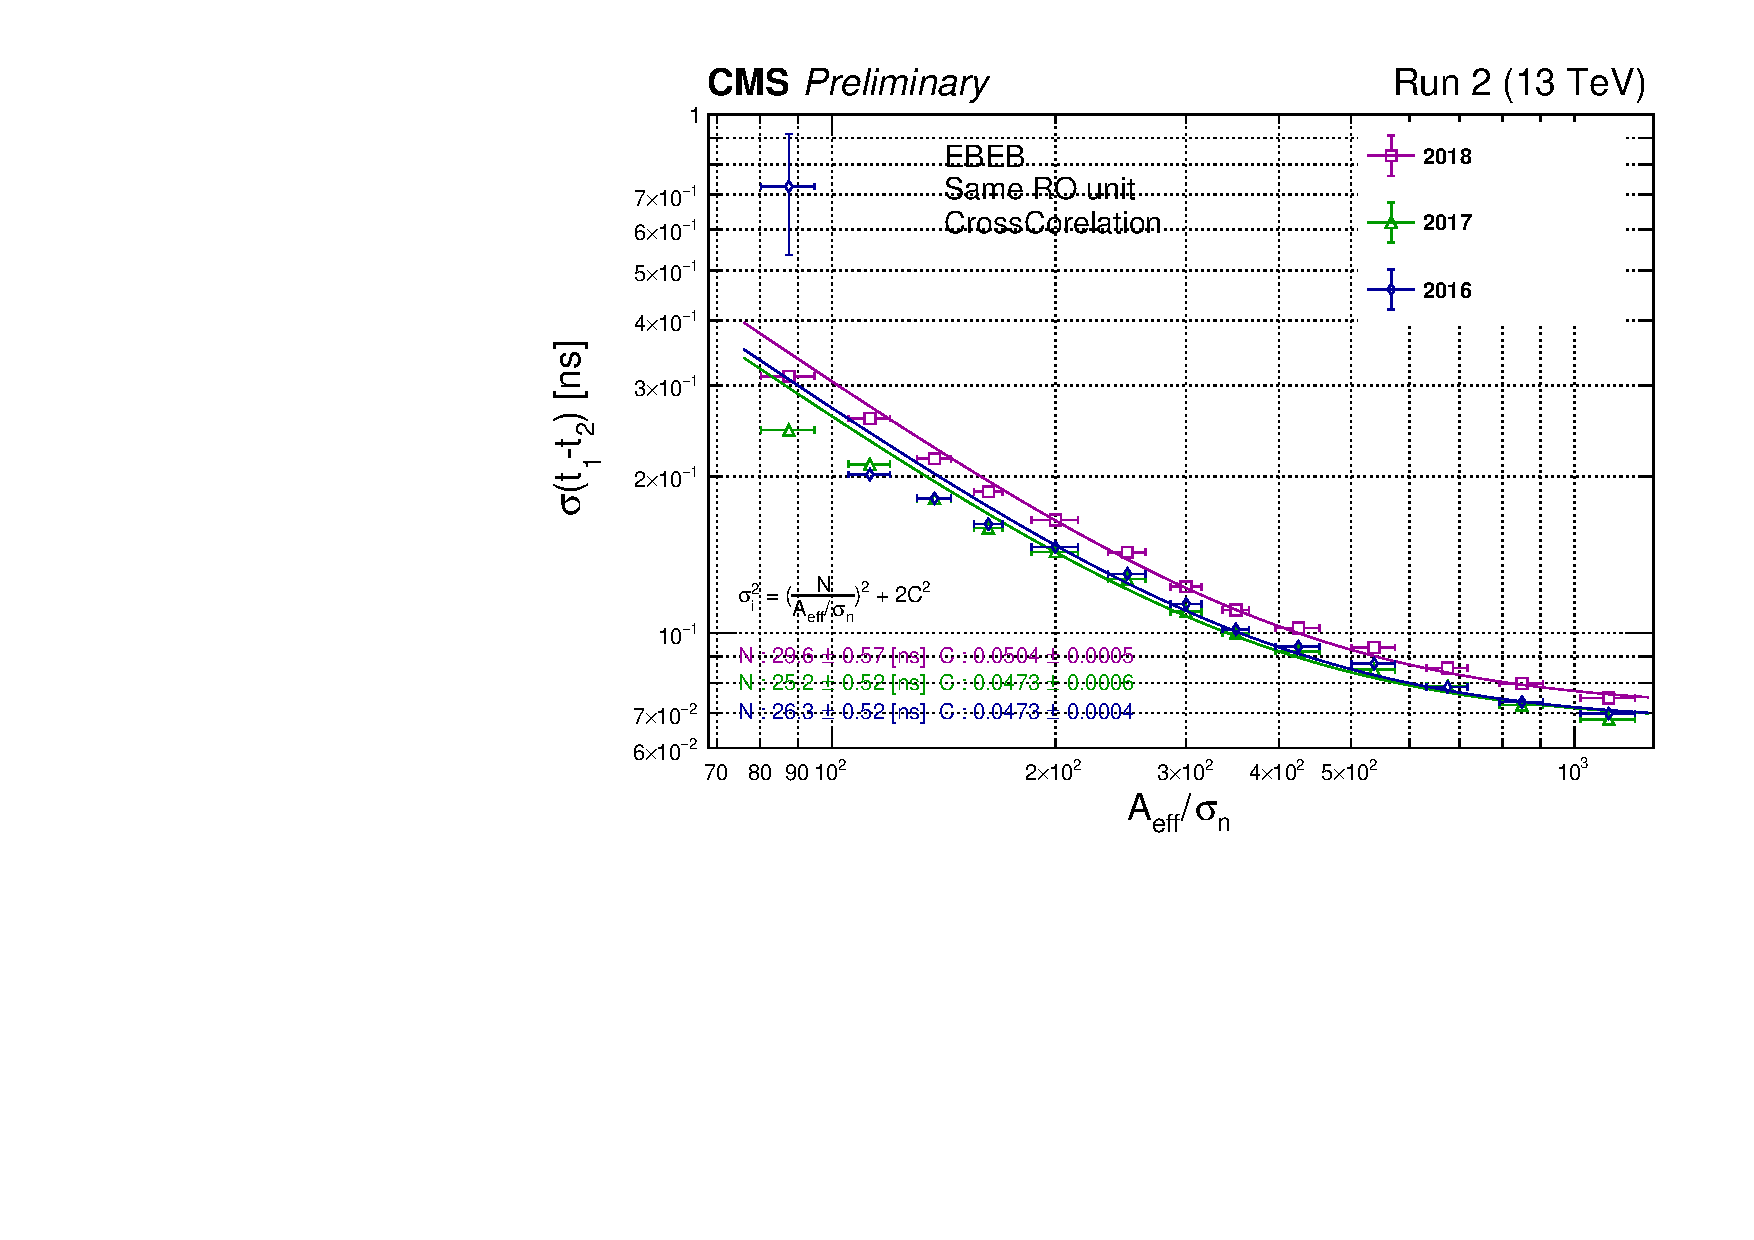
\includegraphics{fig/sec_results/tr_kucc_r2_ls_v22_29062021163409.pdf}}
%\resizebox{0.32\textwidth}{!}{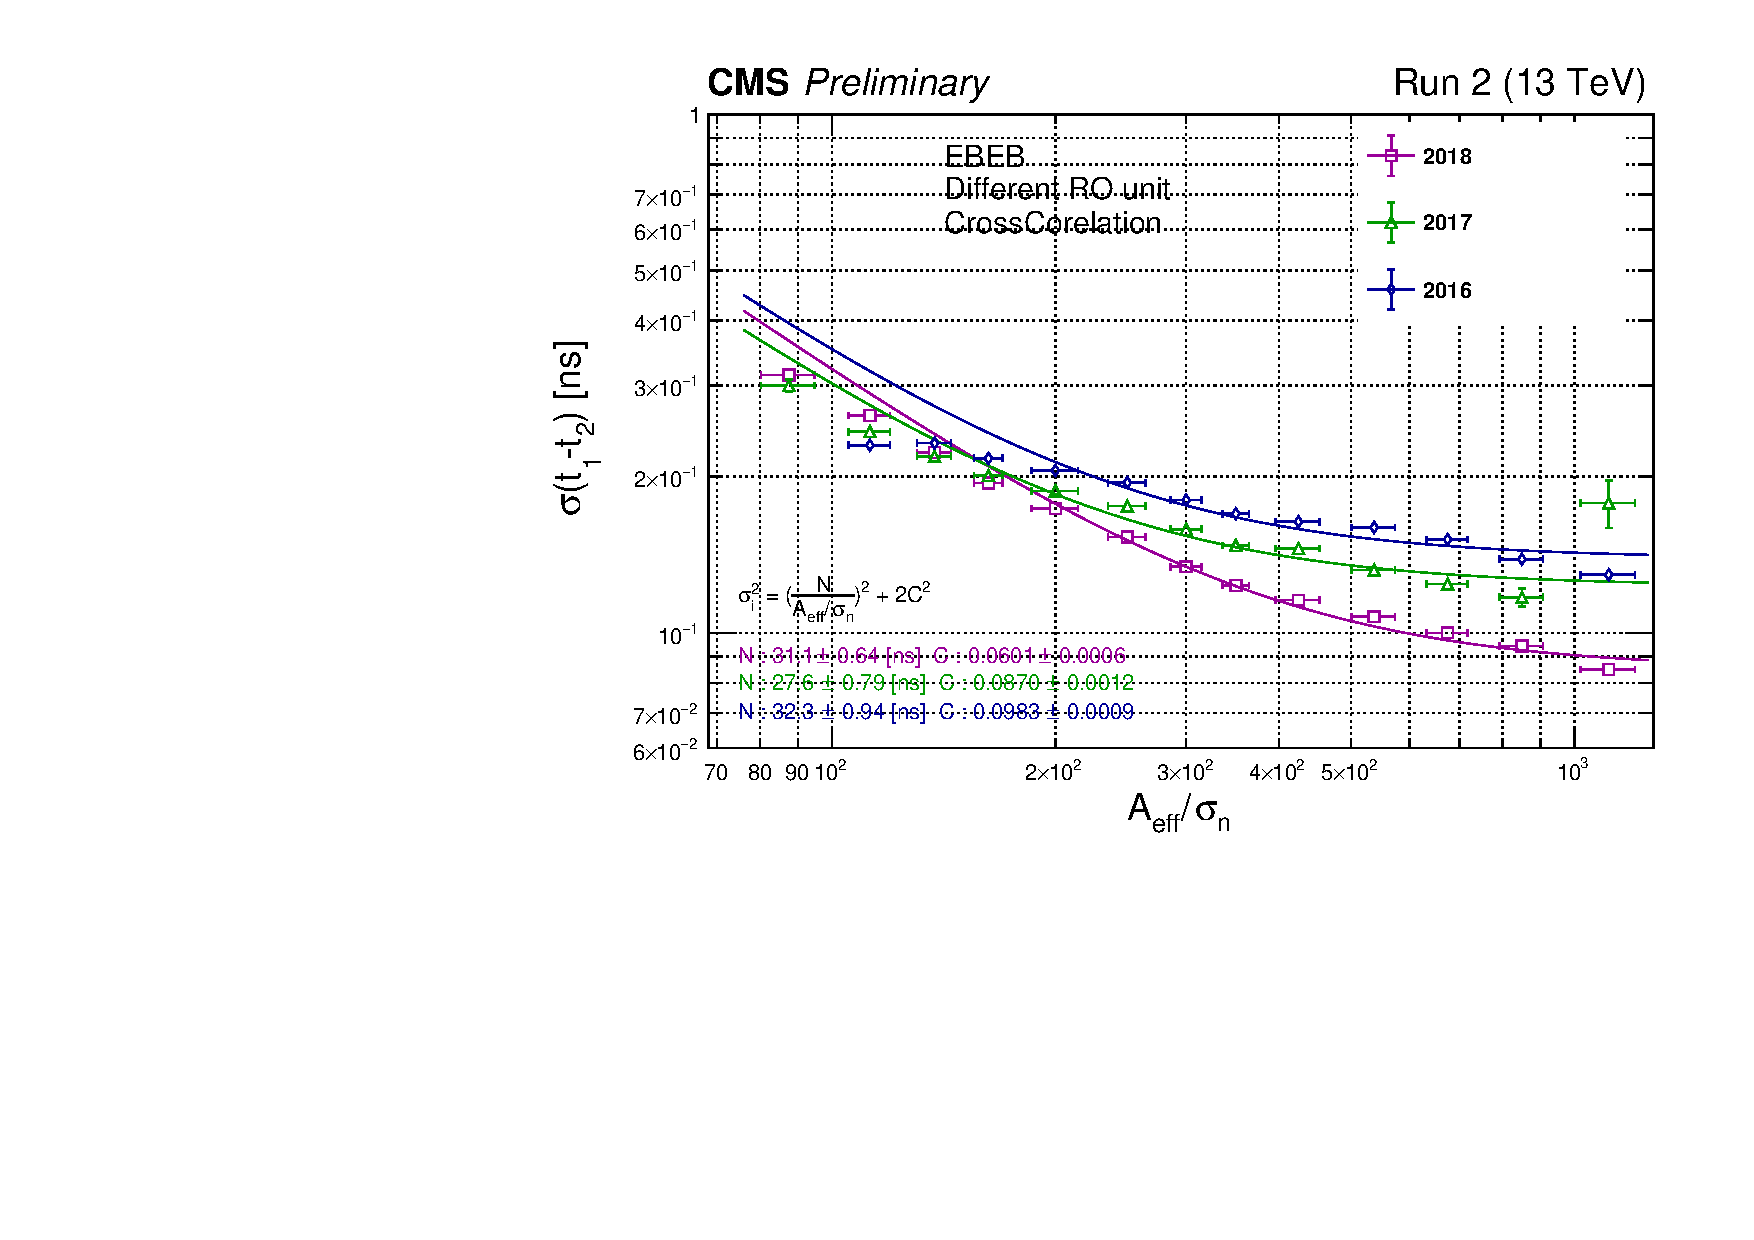
\includegraphics{fig/sec_results/tr_kucc_r2_ld_v22_29062021163409.pdf}}
%\resizebox{0.32\textwidth}{!}{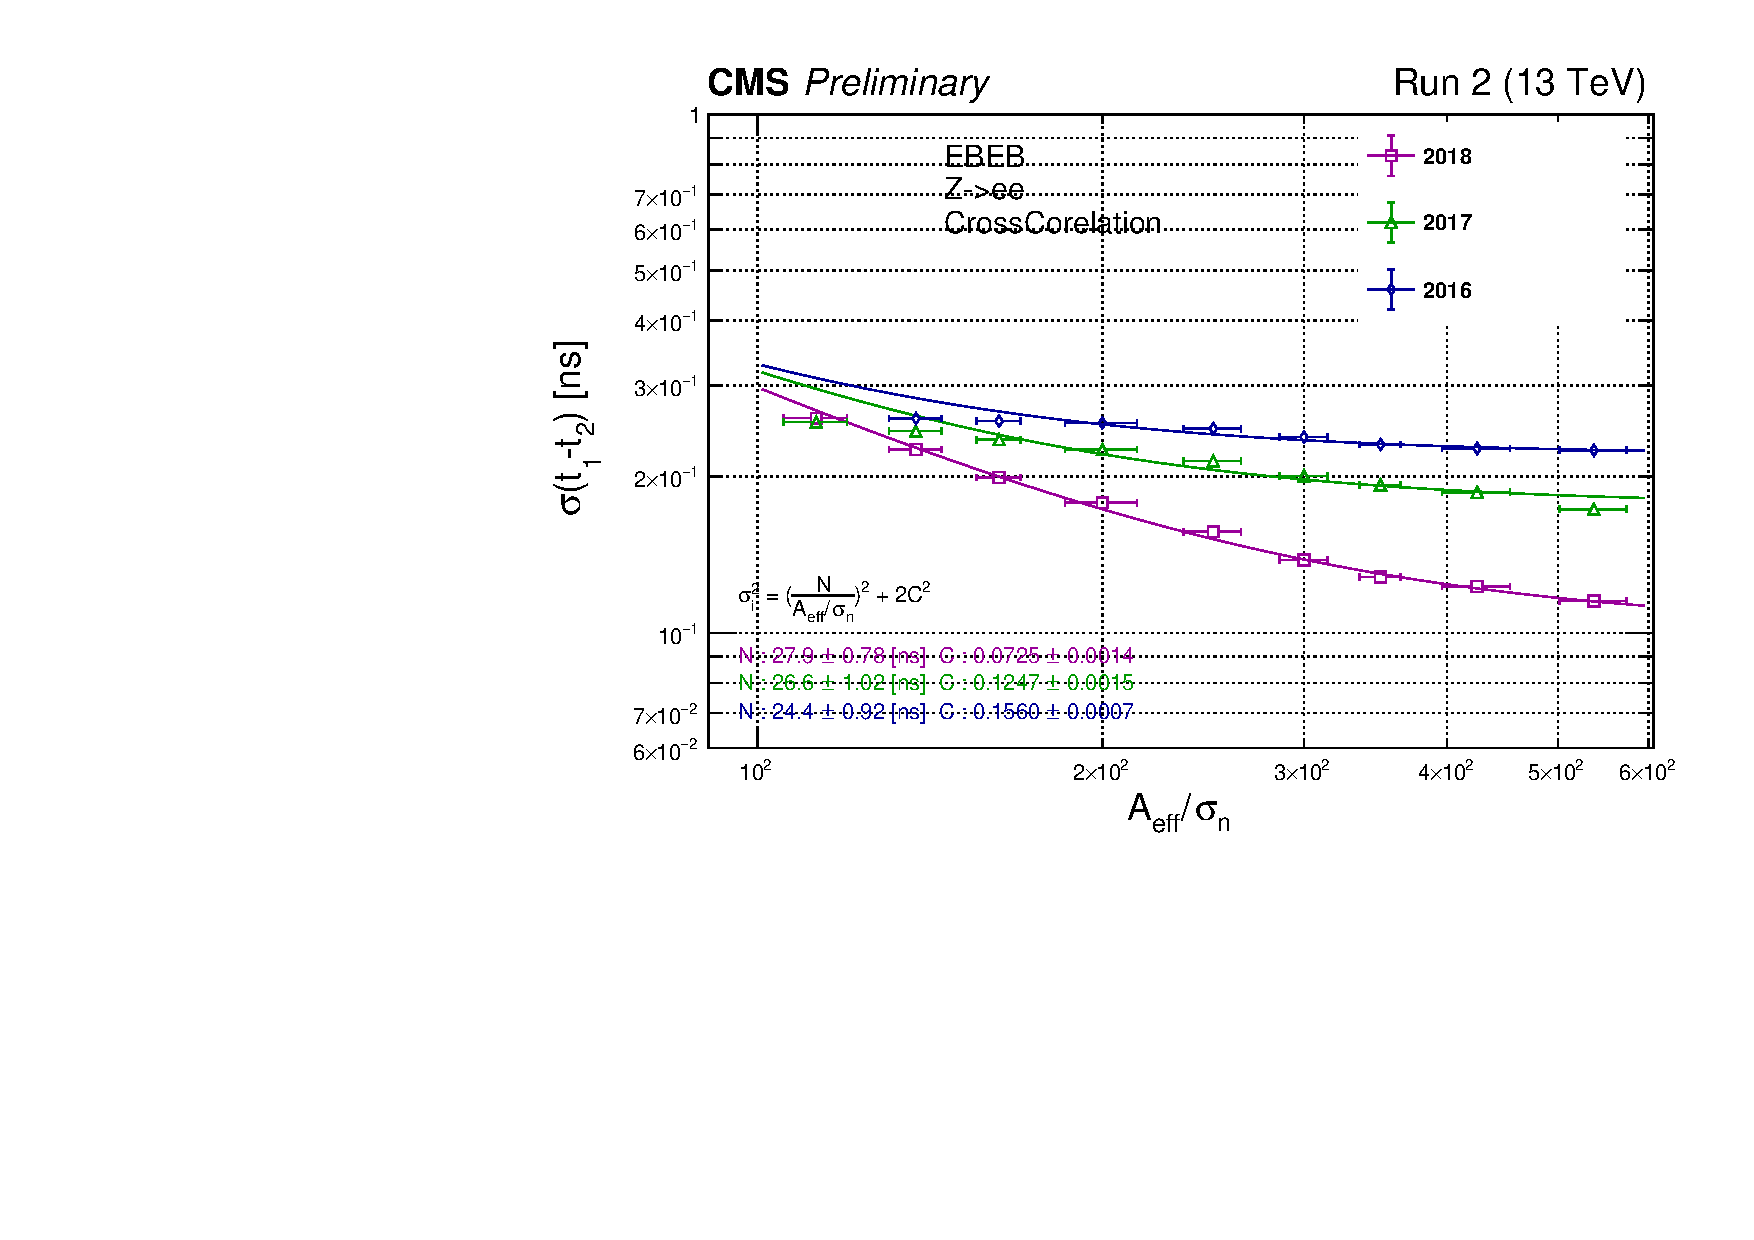
\includegraphics{fig/sec_results/tr_kucc_r2_gi_v22_29062021163757.pdf}}
\resizebox{0.44\textwidth}{!}{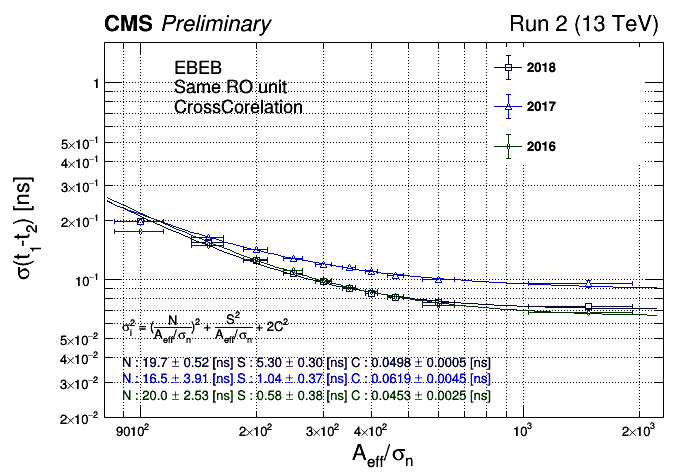
\includegraphics{fig/sec_results/tr_kucc_r2_ls_v25_01122021154153.png}}
\resizebox{0.44\textwidth}{!}{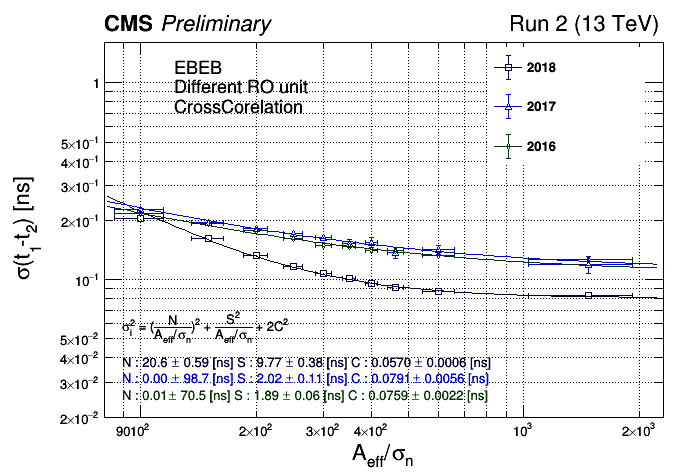
\includegraphics{fig/sec_results/tr_kucc_r2_ld_v25_01122021154153.png}}
\resizebox{0.44\textwidth}{!}{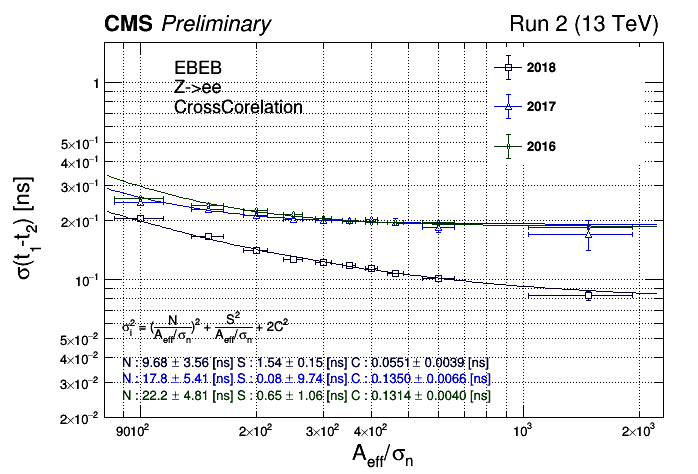
\includegraphics{fig/sec_results/tr_kucc_r2_gi_v25_01122021154153.png}}
\caption{
%ECAL time reconstruction resolution with the cross correlation method Run 2 with in-house calibration applied. 
ECAL reconstruction same RO unit, different RO unit, and $Z\rightarrow e^{+}e^{-}$ KUCC method time resolutions for End of Year Run 2 produced with the EGamma data-stream for 2018 and Double Egamma data-stream for 2017 and 2016 using the 5 GeV offline calibration.}
\label{678CCres}
\end{center}
\end{figure}

\begin{figure}[htbp]
\begin{center}
%\resizebox{0.32\textwidth}{!}{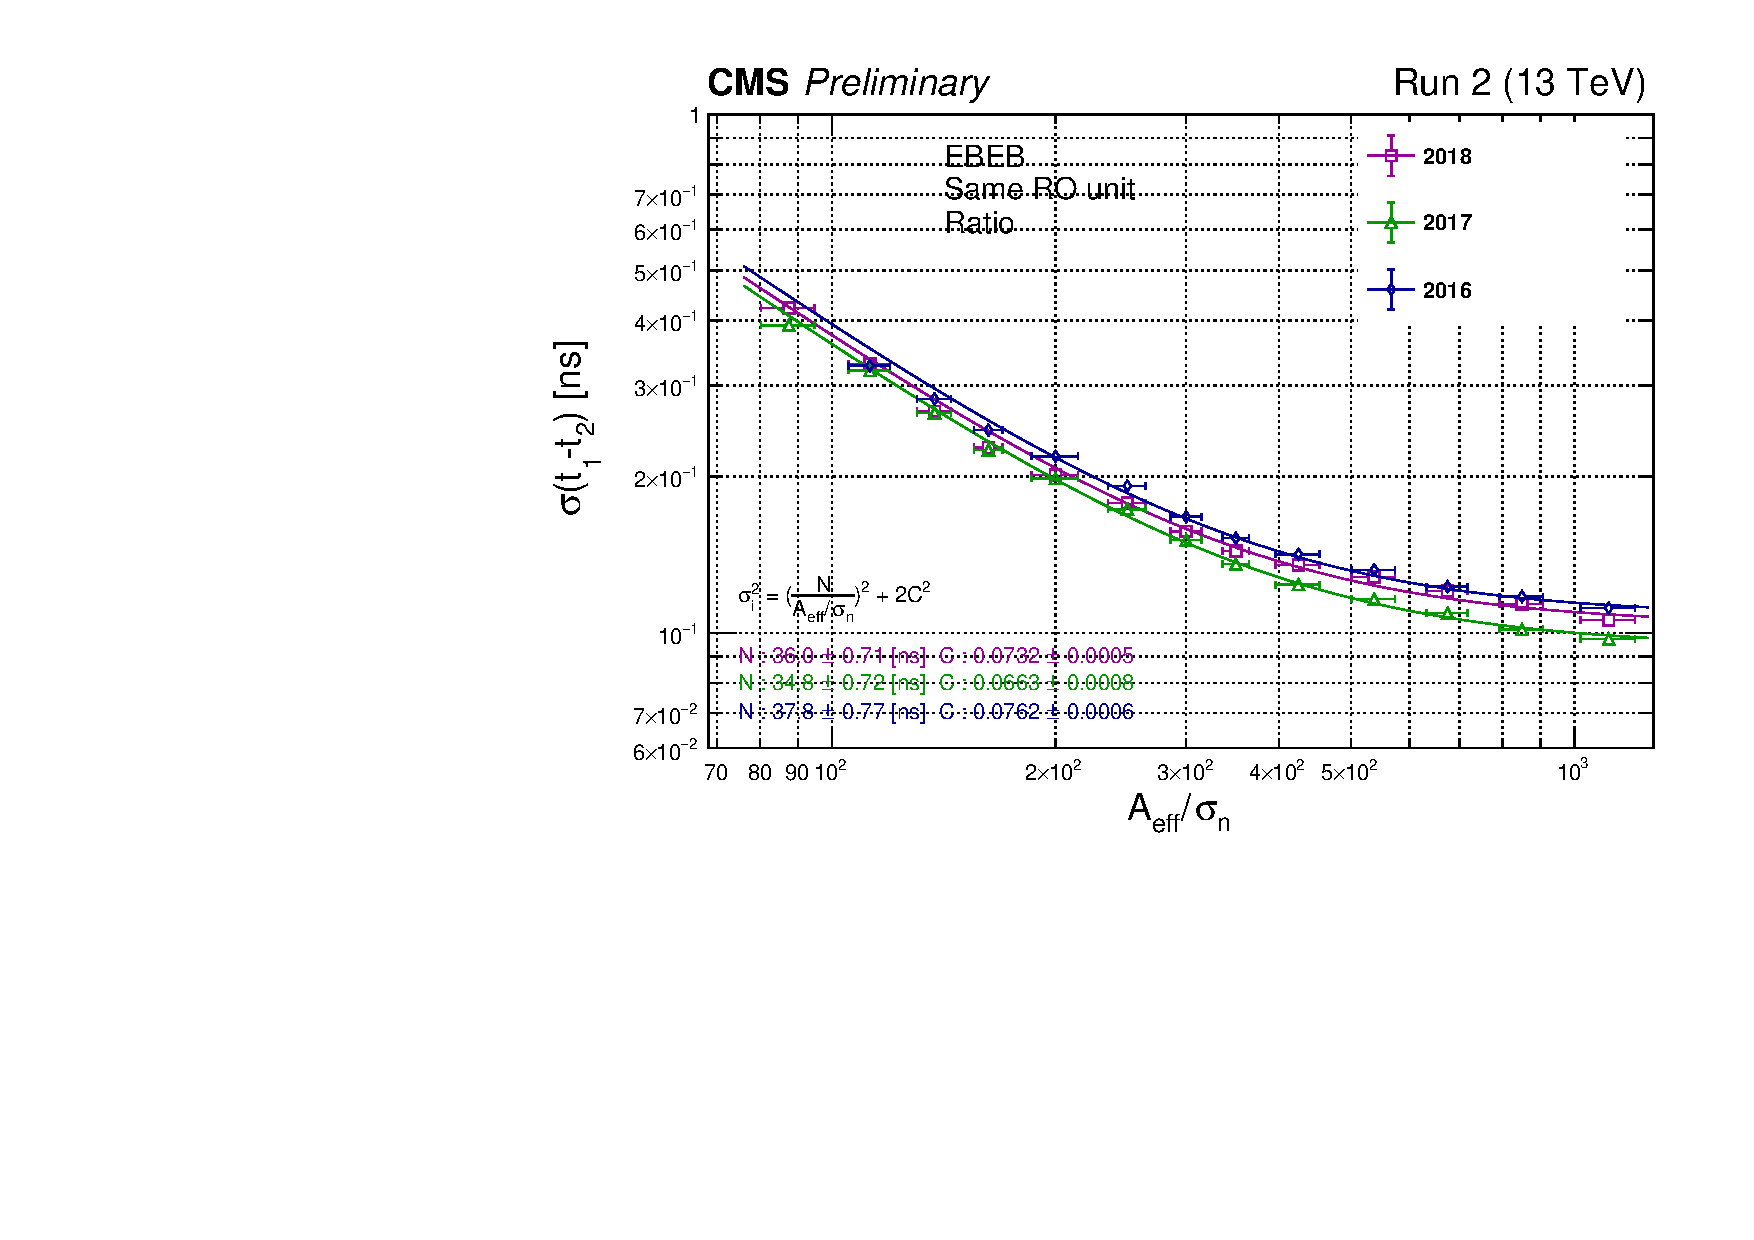
\includegraphics{fig/sec_results/tr_ratio_r2_ls_v22_29062021163409.pdf}}
%\resizebox{0.32\textwidth}{!}{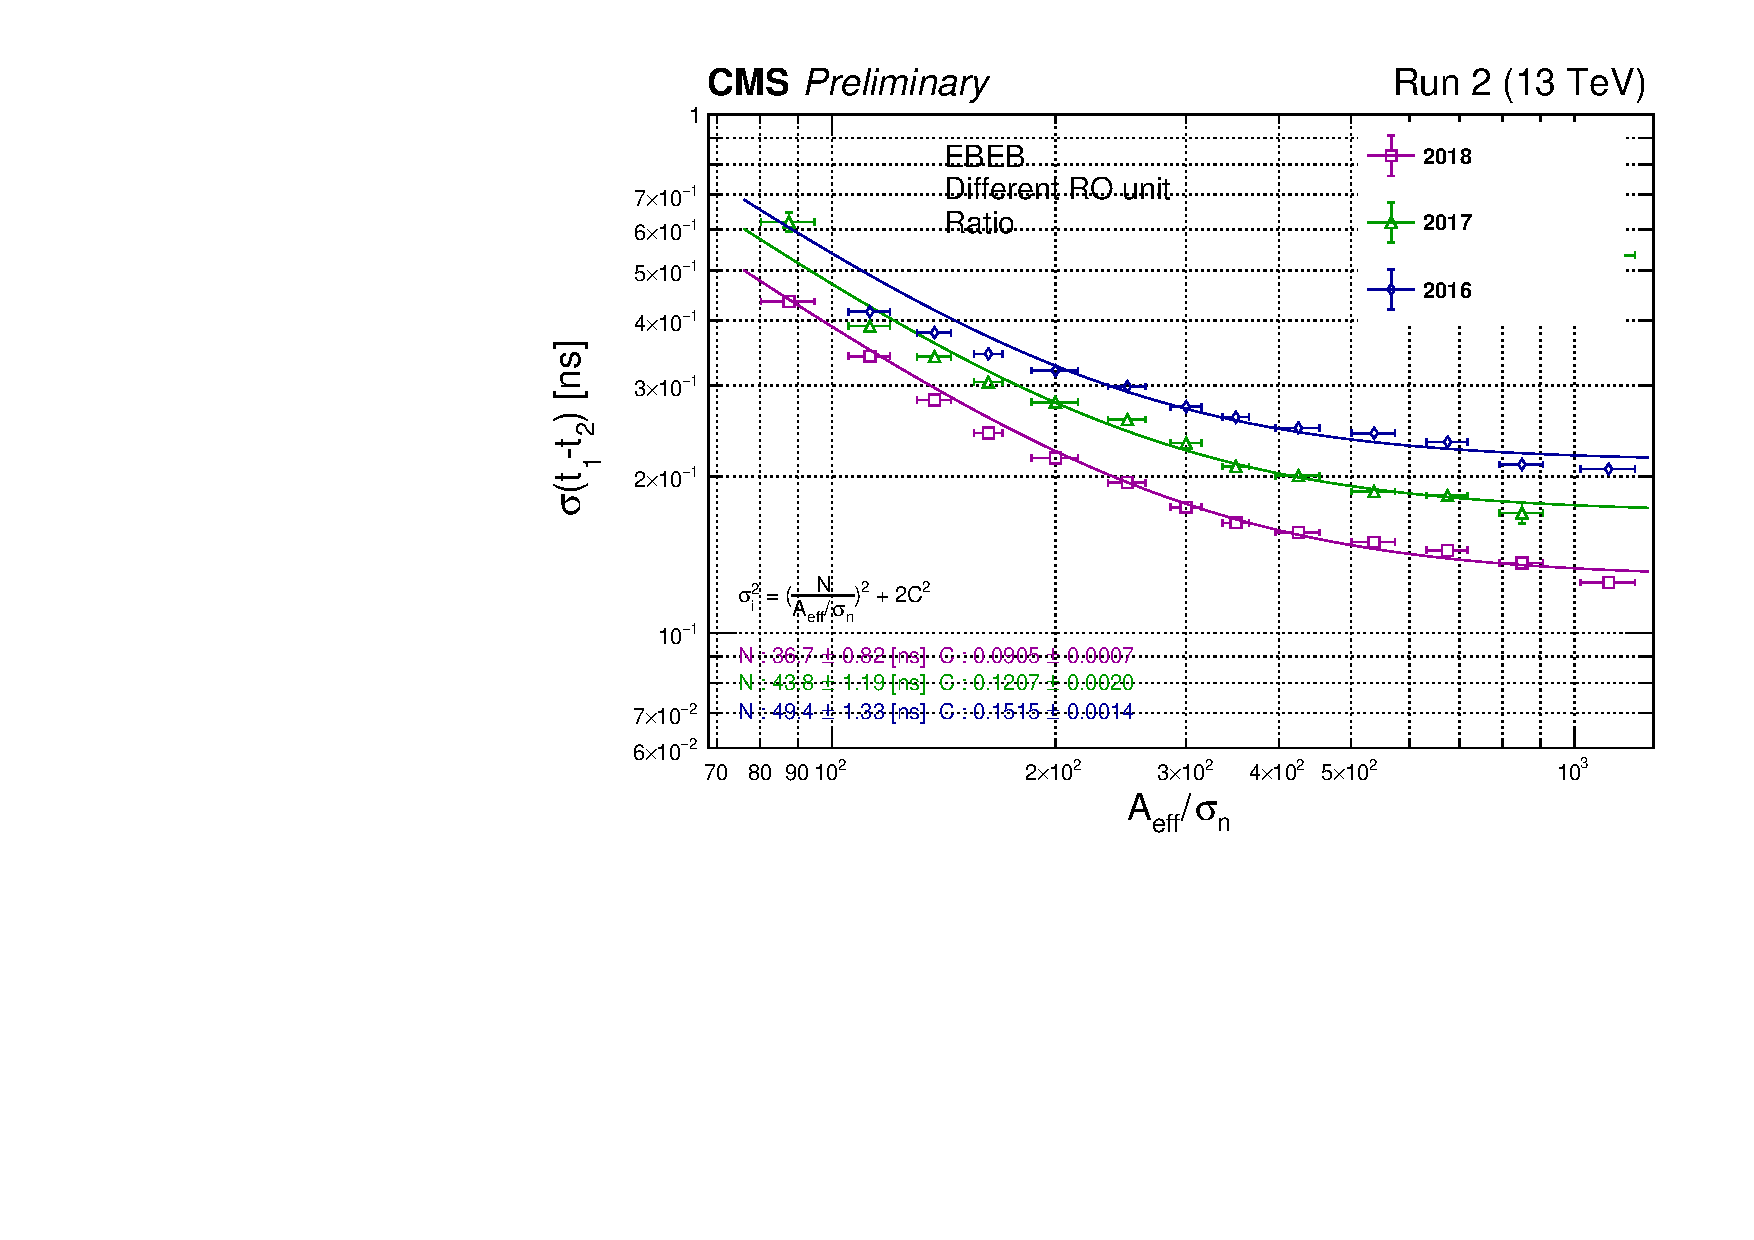
\includegraphics{fig/sec_results/tr_ratio_r2_ld_v22_29062021163409.pdf}}
%\resizebox{0.32\textwidth}{!}{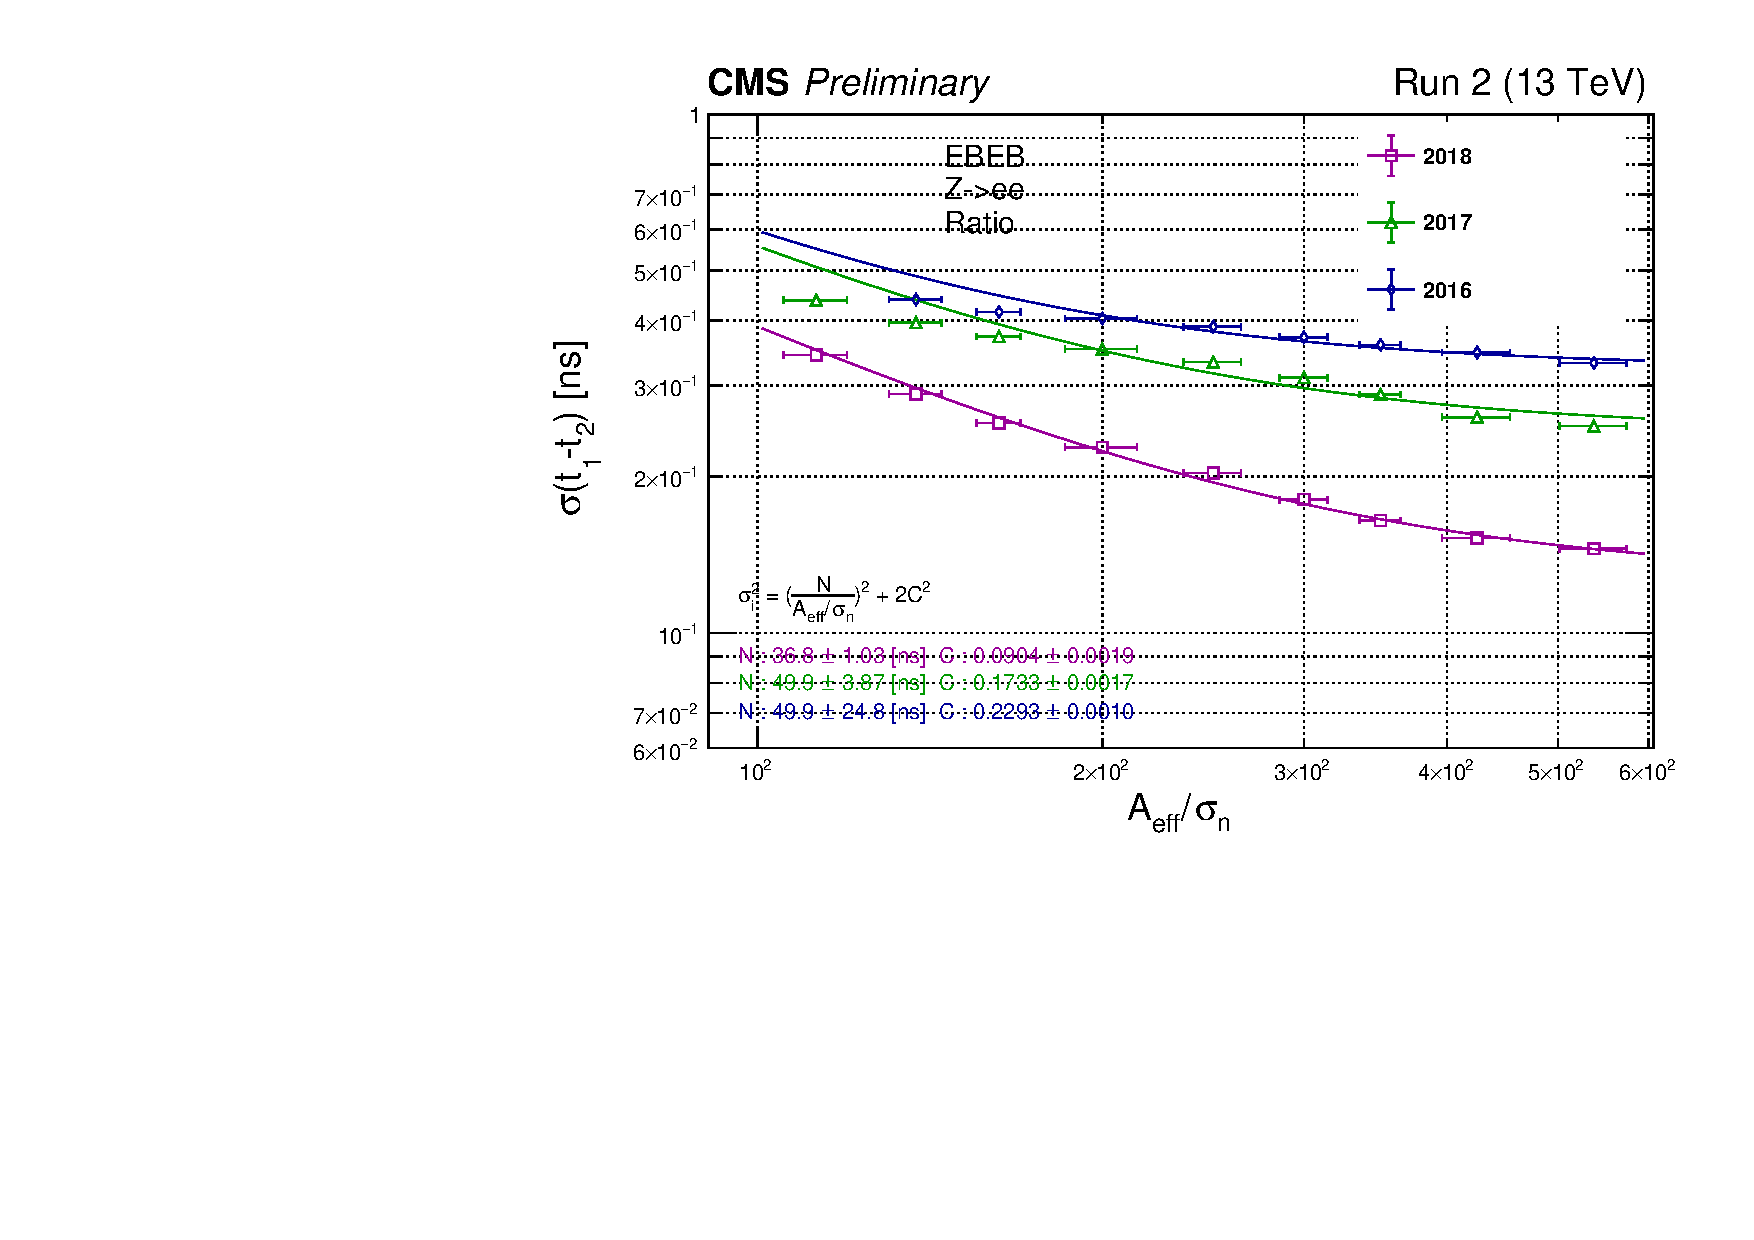
\includegraphics{fig/sec_results/tr_ratio_r2_gi_v22_29062021163757.pdf}}
\resizebox{0.44\textwidth}{!}{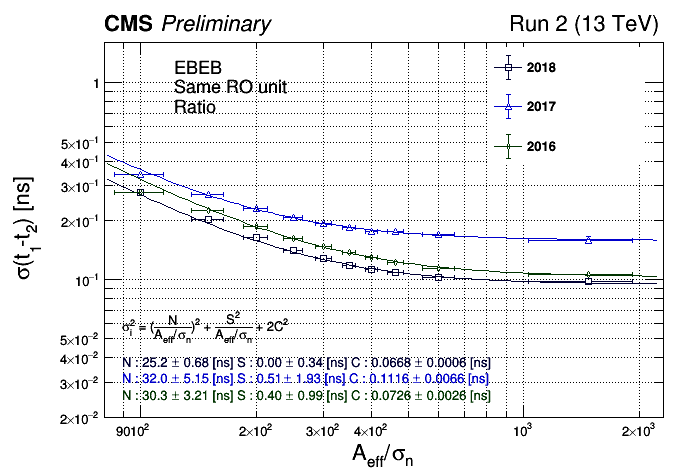
\includegraphics{fig/sec_results/tr_ratio_r2_ls_v25_01122021154153.png}}
\resizebox{0.44\textwidth}{!}{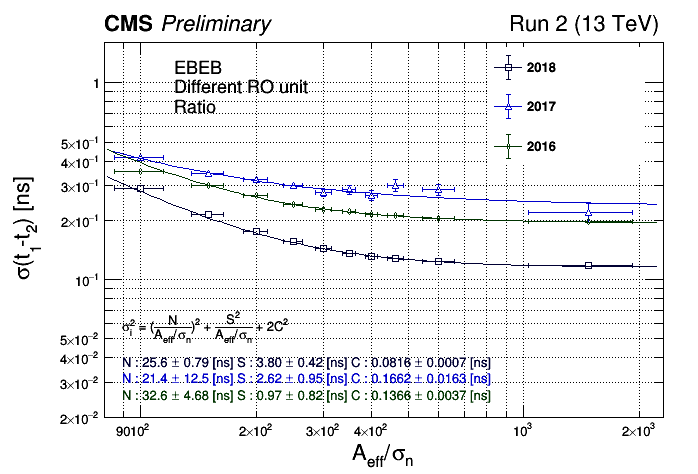
\includegraphics{fig/sec_results/tr_ratio_r2_ld_v25_01122021154153.png}}
\resizebox{0.44\textwidth}{!}{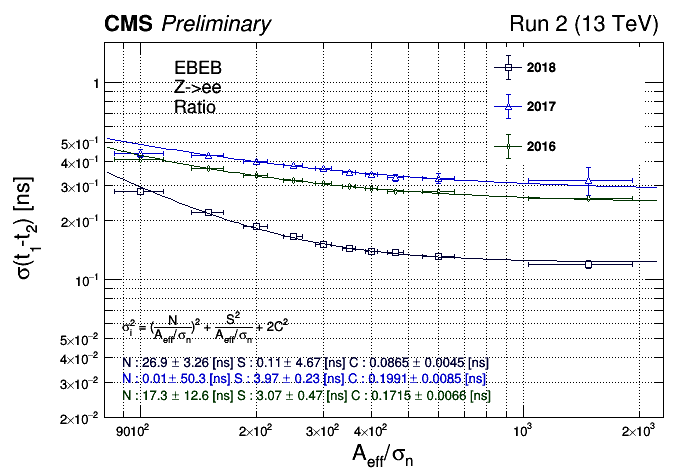
\includegraphics{fig/sec_results/tr_ratio_r2_gi_v25_01122021154153.png}}
\caption{
%ECAL time reconstruction resolution with the ratio method Run 2 with in-house calibration applied.
ECAL reconstruction same RO unit, different RO unit, and $Z\rightarrow e^{+}e^{-}$ Ratio method time resolutions for End of Year Run 2 produced with the EGamma data-stream for 2018 and Double Egamma data-stream for 2017 and 2016 using the 5 GeV offline calibration.}
\label{678e5Ratiores}
\end{center}
\end{figure}

%\begin{table}[htbp]
\begin{center}
 \begin{tabular}{ |c|c|c|c| }
 \multicolumn{4}{c}{                            } \\
 \hline
 \multicolumn{4}{|c|}{  Same RO Unit  }\\
 \hline
 Era & N & S & C \\
 \hline
 \hline
 \multicolumn{4}{|c|}{Ratio}\\
 \hline
 2018 & 25.2 $\pm$ 0.68 & 0.00 $\pm$ 0.34 & 0.0668 $\pm$ 0.0006 \\
 2017 & 32.0 $\pm$ 5.15  & 0.51 $\pm$ 1.93 & 0.1116 $\pm$ 0.0066 \\
 2016 & 30.3 $\pm$ 3.21 & 0.40 $\pm$ 0.99 & 0.0726 $\pm$ 0.0026 \\
 \hline
 \multicolumn{4}{|c|}{Cross Correlation}\\
 \hline
 2018 & 19.7 $\pm$ 0.52 & 5.30 $\pm$ 0.30 & 0.0498 $\pm$ 0.0005 \\
 2017 & 16.5 $\pm$ 3.91 & 1.04 $\pm$ 0.37 & 0.0619 $\pm$ 0.0045 \\
 2016 & 20.0 $\pm$ 2.53 & 0.58 $\pm$ 0.38 & 0.0453 $\pm$ 0.0025 \\
 \hline
 \end{tabular}
\end{center}
%\end{table}
 
%\begin{table}[htbp]
 \begin{center}
 \begin{tabular}{ |c|c|c|c| }
 \multicolumn{4}{c}{                            } \\
 \hline
  \multicolumn{4}{|c|}{Different RO Unit}\\
 \hline
 Era & N & S & C \\
 \hline
 \multicolumn{4}{|c|}{Ratio}\\
 \hline
 2018 & 25.6 $\pm$ 0.79 & 3.80 $\pm$ 0.42 & 0.0816 $\pm$ 0.0007 \\
 2017 & 21.4 $\pm$ 12.5 & 2.62 $\pm$ 0.95 & 0.1662 $\pm$ 0.0163 \\
 2016 & 32.6 $\pm$ 4.68 & 0.97 $\pm$ 0.82 & 0.1366 $\pm$ 0.0037 \\
 \hline
 \multicolumn{4}{|c|}{Cross Correlation}\\
 \hline
 2018 & 20.6 $\pm$ 0.59 & 9.77 $\pm$ 0.38 & 0.0570 $\pm$ 0.0006 \\
 2017 & 0.00 $\pm$ 98.7 & 2.02 $\pm$ 0.11 & 0.0791 $\pm$ 0.0056 \\
 2016 & 0.01 $\pm$ 70.5 & 1.89 $\pm$ 0.06 & 0.0759 $\pm$ 0.0022 \\
 \hline
\end{tabular}
\end{center}
%\end{table}

%\begin{table}[htbp]
\begin{center}
 \begin{tabular}{ |c|c|c|c| }
 \multicolumn{4}{c}{                            } \\
 \hline
  \multicolumn{4}{|c|}{$Z\rightarrow e^{+}e^{-}$}\\
 \hline
 Era & N & S & C \\
 \hline
 \multicolumn{4}{|c|}{Ratio}\\
 \hline
 2018 & 26.9 $\pm$ 3.26 & 0.11 $\pm$ 4.67 & 0.0865 $\pm$ 0.0045 \\
 2017 & 0.01 $\pm$ 50.3 & 3.97 $\pm$ 0.23 & 0.1991 $\pm$ 0.0085 \\
 2016 & 17.3 $\pm$ 12.6 & 3.07 $\pm$ 0.47 & 0.1715 $\pm$ 0.0066 \\
 \hline
 \multicolumn{4}{|c|}{Cross Correlation}\\
 \hline
 2018 & 9.68 $\pm$ 3.56 & 1.54 $\pm$ 0.15 & 0.0551 $\pm$ 0.0039 \\
 2017 & 17.8 $\pm$ 5.41 & 0.08 $\pm$ 9.74 & 0.1350 $\pm$ 0.0066 \\
 2016 & 22.2 $\pm$ 4.81 & 0.65 $\pm$ 1.06 & 0.1314 $\pm$ 0.0040 \\
\hline
\end{tabular}
\end{center}
%\end{table}

\newpage